\documentclass[12pt]{article}
\usepackage[utf8]{inputenc}
\usepackage{graphicx}
\usepackage{hyperref}
\usepackage{apacite}
\usepackage{listings}

% APA Style Cover Page Adjustments
\title{
    \vspace{2in} % Adjust vertical space as needed
    Final Term Project - Google Play Store
    \vspace{1.5in} % Additional vertical space before author name
}
\author{
    Baiyi Zhang \\
    CS 5805: Machine Learning I \\
    Dr. Reza Jafari \\
    \vspace{1.5in} % Additional vertical space before date
    December 7, 2023 \\% Replace with specific date if necessary 
}
\date{} % Empty date to avoid duplication

\begin{document}

% Create the title page
\maketitle
\thispagestyle{empty} % No header or footer on title page
\newpage
\pagenumbering{roman}
\tableofcontents
\newpage
\listoffigures
\newpage
\pagenumbering{arabic}
% Include sections
\section{Abstract}
% Your abstract text goes here.

\section{Introduction}
The project is divided into 4 phases.

Phase 1 starts with cleaning N/A values and duplicates of the dataset, followed by feature importance analyzing and principle component analysis to reduce dimensionality. Normal transformation and standardization are applied to detect and remove outliers. Finally, correlation matrix suggest that collinearity does not exist in the dataset.

Phase 2 uses dataset generated by phase 1 to make predictions on a continuous numerical feature, number of installs, using a multiple linear regression model. As backward step-wise analysis failed to estimate meaningful regression model, random forest regressor proves to have a better fit based on MSE and $R^2$.

Phase 3 programmed a pipeline to analyze metrics and plot ROC curve of classifiers include decision tree, logistic regression, KNN, SVM, Na\"ive Bayes, Random Forest, Stacking, Boosting and Neural Network. The hyper parameter for each classifier is obtained by grid search with cross validation. Comparing the precision, recall, specificity, F score and ROC, the best model is Neural Network Classifier for performing better in AUC without compromising F score and precision.

Phase 4 uses K-means and DBSCAN to cluster the observations of the dataset and visualized the result using PCA. Optimal K is obtained by elbow method and silhouette analysis. Phase 4 also applies Apriori algorithm to find association rules among dataset.
\section{Description of the Dataset}
% Description of your dataset goes here.

\section{Phase 1 - Feature Engineering \& EDA}
% Description of your dataset goes here.
\subsection{Data Cleaning}

\subsubsection{Raw data overview}
Figure~\ref{fig:raw-data} contains the percentage of non-applicable (N/A) data and the uniqueness of each original feature. During the forthcoming stages of analysis and data cleansing, certain unique identifiers, such as \texttt{app\_id}, might be discarded due to their limited informative value. \texttt{minimum\_installs} and \texttt{maximum\_installs} represent two distinct aspects of installation counts: the former indicates a range, whereas the latter provides a precise, continuous figure. In subsequent steps, I will conduct a series of operations to evaluate the relevance of each feature, making essential modifications to optimize the data for the training process.

\begin{figure}
    \centering
    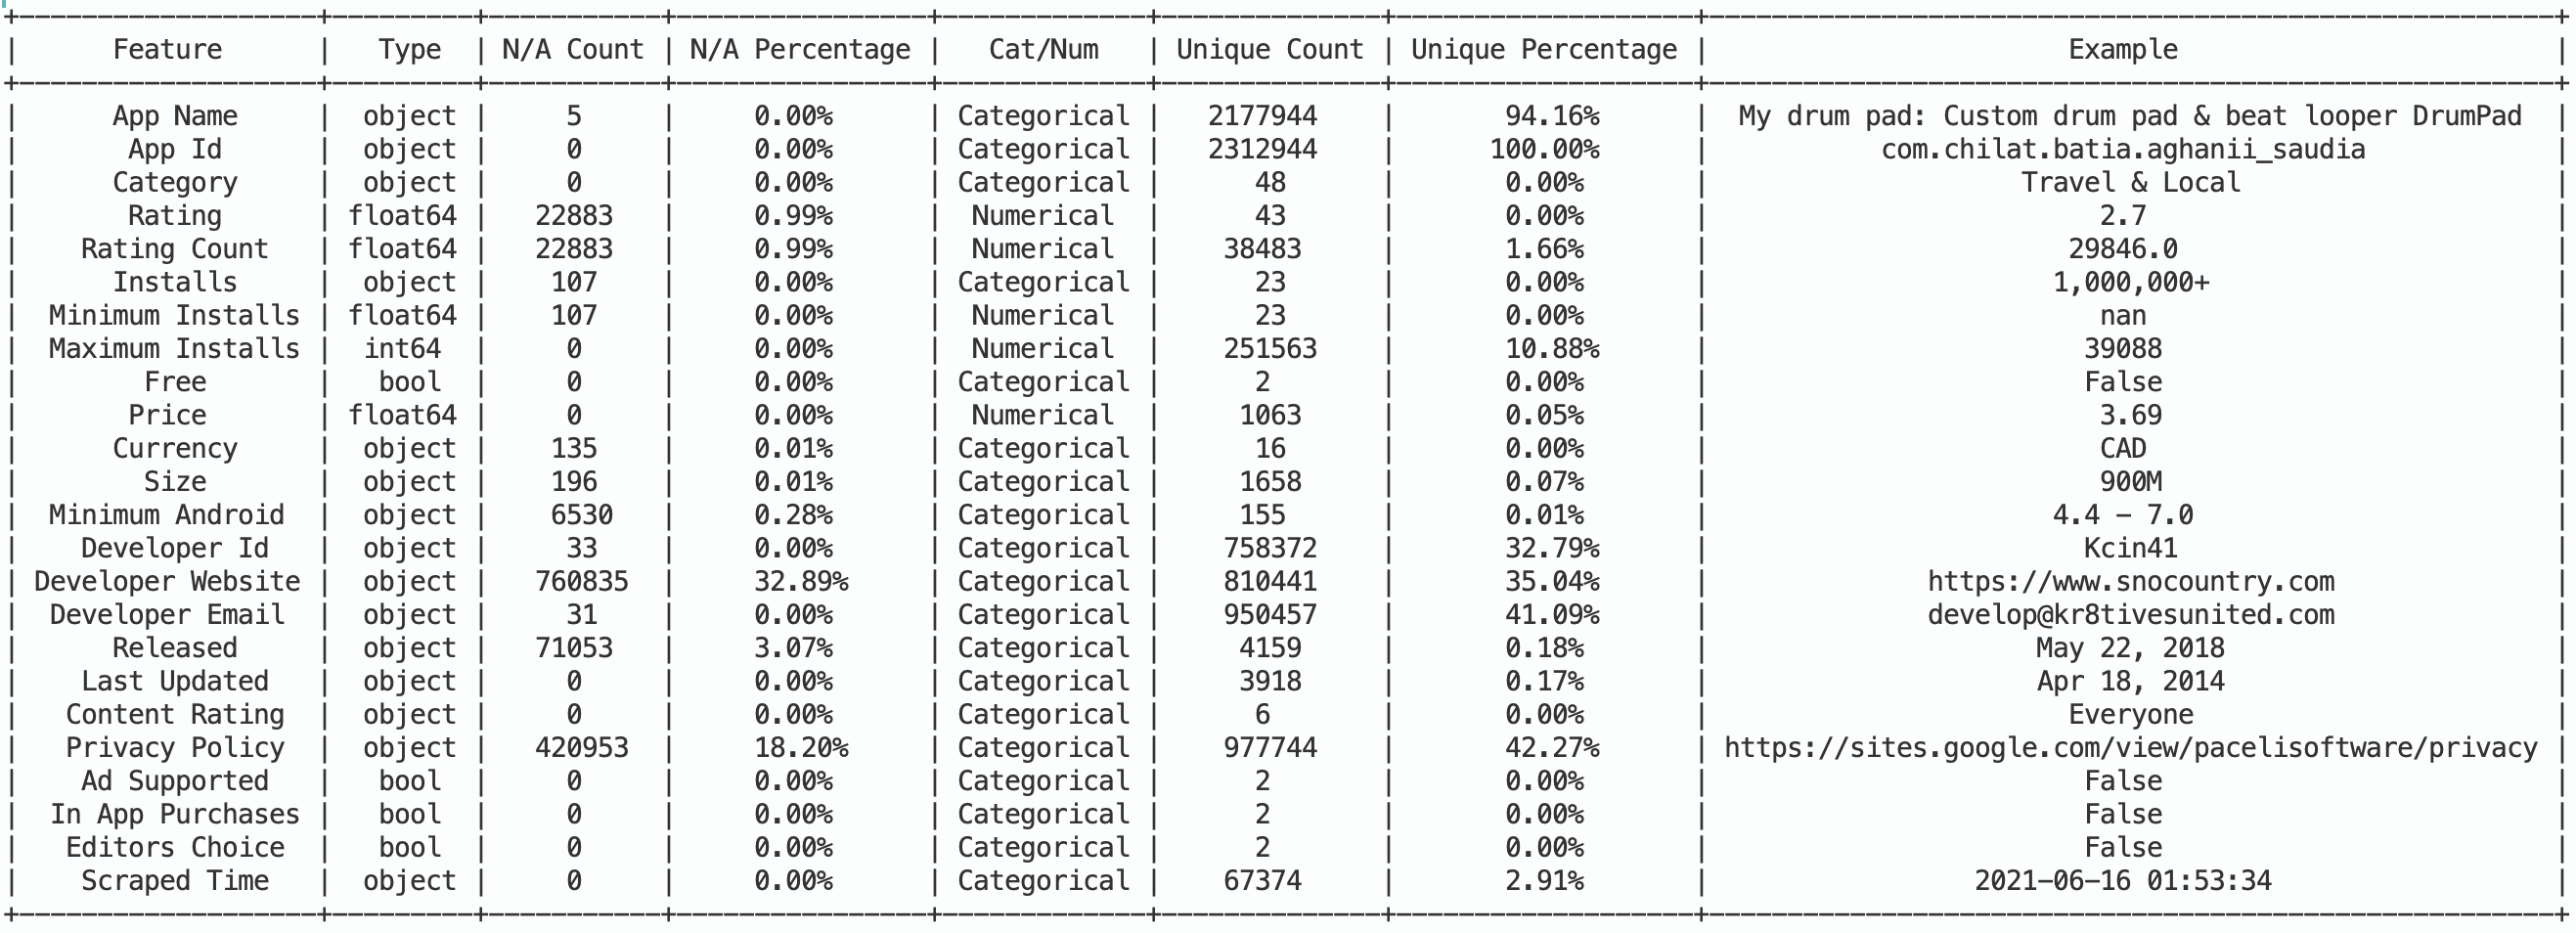
\includegraphics[width=1\linewidth]{docs//assets/raw-data-overview.png}
    \caption{Raw Data Overview}
    \label{fig:raw-data}
\end{figure}

\subsubsection{N/A values percentage}
For Developer Website and Privacy Policy, due to high observation of N/A values, removing the features makes more sense than removing rows with N/A values.

\subsection{Data Duplication}

\subsubsection{Duplication in Currency column}

\begin{figure}[h]
    \centering
    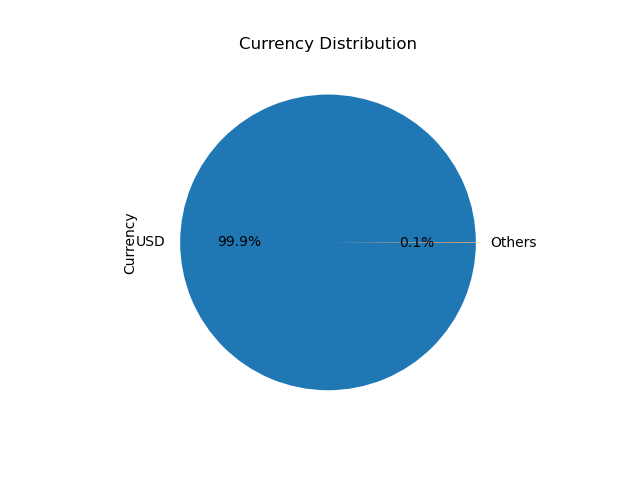
\includegraphics[width=0.8\textwidth]{docs//assets/currency.png}
    \caption{Currency Distribution}
    \label{fig:currency}
\end{figure}

In Figure~\ref{fig:currency}, it is evident that the USD currency represents over 99.9\% of the dataset. By removing observations in other currencies and subsequently deleting the Currency column, we can retain 99.9\% of the data while effectively reducing its dimensionality. This approach streamlines the dataset, focusing on the predominant currency for a more efficient analysis.

\subsubsection{Duplication between Installs and Minimum Installs}
The dataset contains three columns related to app installations, each named with variations of the word Installs. Upon examination, \texttt{maximum\_installs} is found to be a continuous numerical value, whereas Installs and \texttt{minimum\_installs} represent a range, indicating the number of app downloads. Additionally, the Installs column includes characters such as \texttt{+} and \texttt{,}(comma). These issues are now fixed.

\subsubsection{Duplication between Free and Price}
Given that the price of free items is listed as 0, the Free column becomes redundant and has therefore been removed from the dataset.

\subsection{Aggregation}
\subsubsection{Aggregation of Android versions}
The \texttt{minimum\_android} column comprises 27 unique values, each representing a different Android version required for the app's operation. These versions are strings that are not likely to be encoded, such as \texttt{4.1.2}. Given that variations in minor versions do not significantly enhance the analysis of this dataset, a more effective approach is to aggregate these versions by their major numbers (e.g., 4, 5, etc.).

\subsection{Down Sampling}
\subsubsection{Slicing the dataset}
The dataset has a wide range of data distribution. Install count that is extremely low or high is not the main focus of this analysis. As a result, a slice of data that \texttt{installCount} is \textbf{between 100k and 10M} is extracted for analysis.

\subsection{Dimensionality Reduction}
\subsubsection{Random Forest Analysis}

\begin{figure}[h]
    \centering
    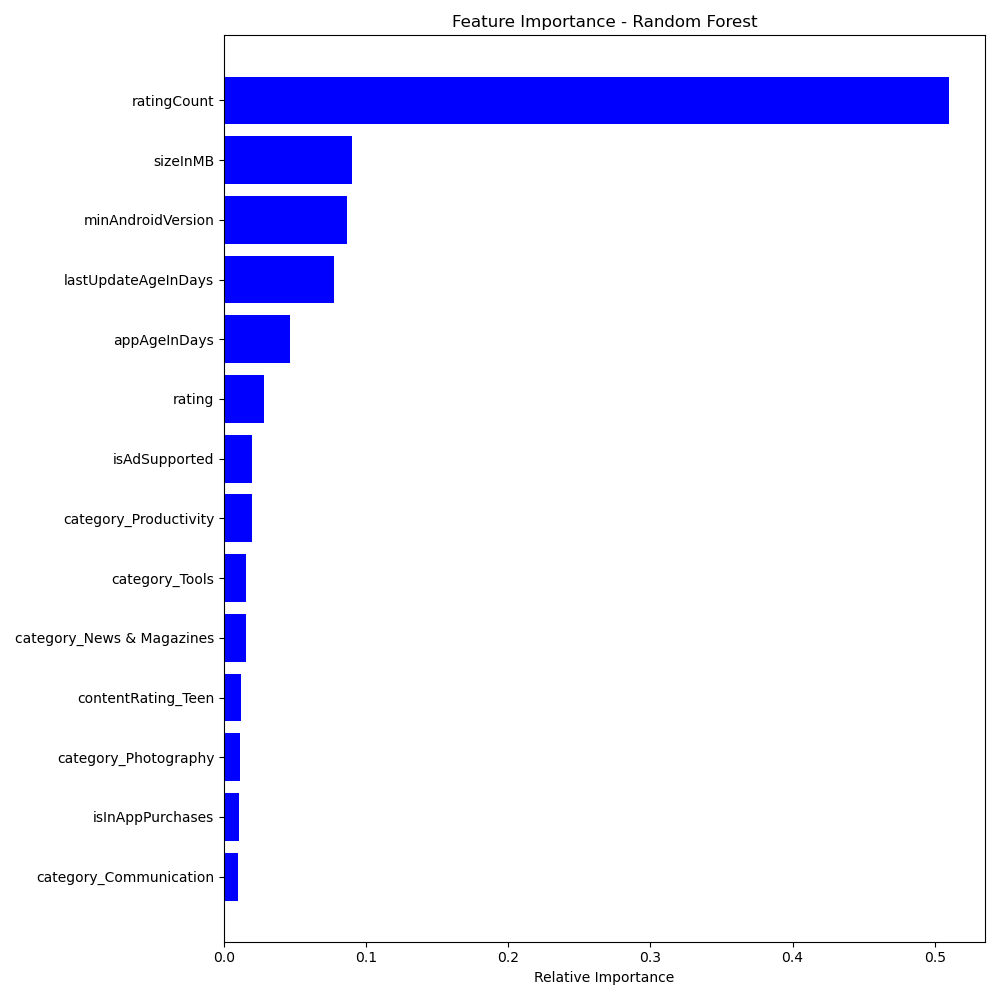
\includegraphics[width=\textwidth]{docs//assets/rfa.png}
    \caption{Feature Importance - Random Forest Analysis}
    \label{fig:rfa}
\end{figure}

The horizontal bar plot in Figure~\ref{fig:rfa} allows us to infer that \texttt{rating\_count} is the most significant feature, followed by \texttt{size\_in\_mb}, \texttt{min\_android\_version}, \texttt{last\_update\_age\_in\_days}, and \texttt{app\_age\_in\_days}. This insight, derived from the Random Forest Analysis, guides subsequent preprocessing steps, aiding in decisions regarding the inclusion or exclusion of specific features.

\subsubsection{Principle Component Analysis and Condition Number}
Figure~\ref{fig:pca} demonstrates that a combination of 10 features cumulatively accounts for 85\% of the variance. The dataset, transformed through PCA, consists of 68 columns, reduced from the original 71. This reduction is likely due to the application of \texttt{pd.get\_dummies} on three features, suggesting that PCA has effectively discarded three columns whose information is captured by the remaining data.

\begin{figure}[h]
    \centering
    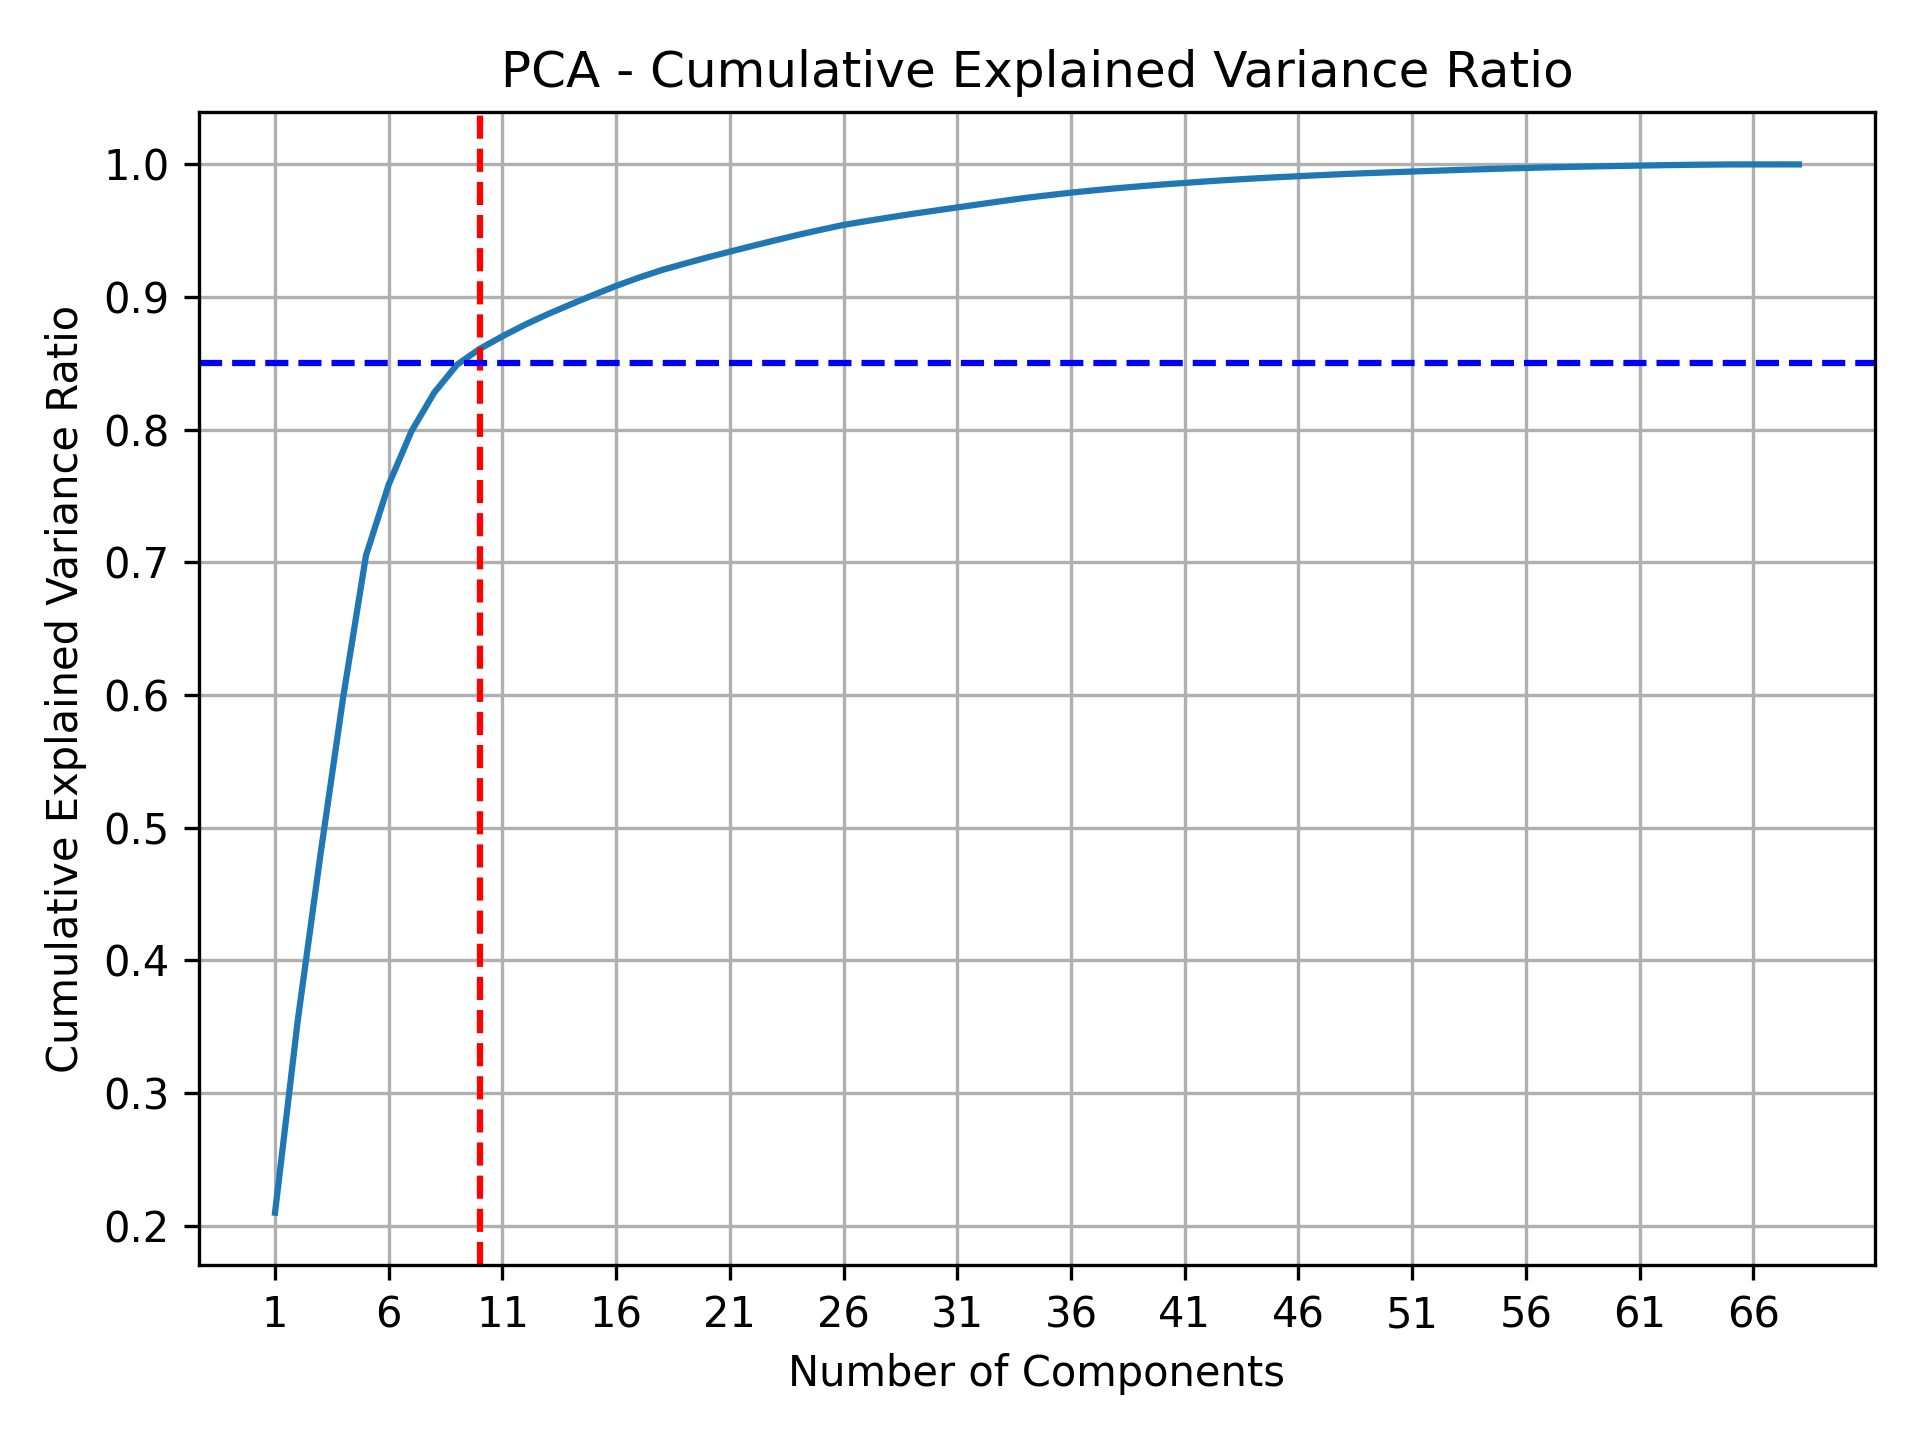
\includegraphics[width=\textwidth]{docs//assets/pca.png}
    \caption{Explained Variance Ratio - PCA}
    \label{fig:pca}
\end{figure}

The program additionally computed the condition number. Prior to the PCA transformation, the condition number was exceedingly high. However, following the transformation, it significantly reduced to 164.65. This decrease in the condition number implies that potential collinearity has been eliminated. Such collinearity might have originated from the use of the \texttt{get\_dummies} method.


\begin{center}
    Comparison of Condition Number
\begin{table}[ht]
\centering
    \begin{tabular}{cc}
        \toprule
        Original & PCA Transformed \\
        \midrule
        75869592332155.22 & 164.65 \\
        \bottomrule
    \end{tabular}
\end{table}
\end{center}


\subsubsection{Singular Value Decomposition Analysis}

\begin{figure}[h]
\centering
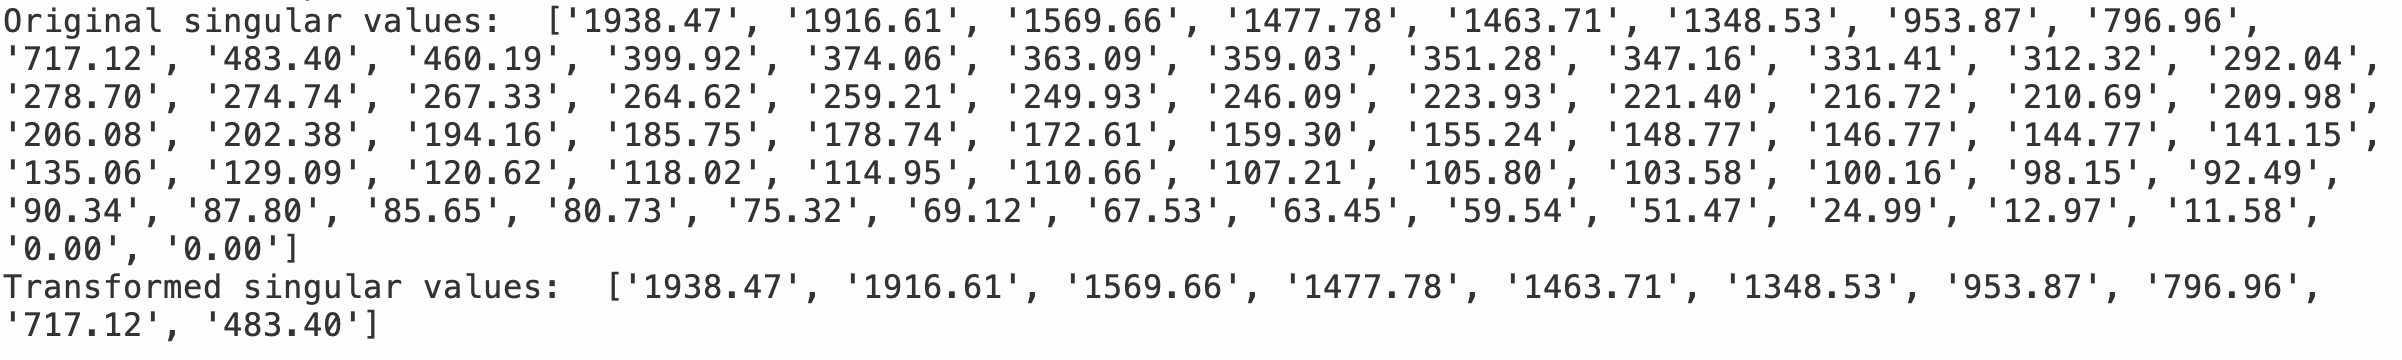
\includegraphics[width=\textwidth]{docs//assets/svd.png}
\caption{Singular Values of Data}
\end{figure}

Following the PCA analysis, 10 features were chosen for the SVD transformation. Figure X presents a comparison of the dataset's singular values before and after the SVD transformation. It is observed that the singular values remain consistent throughout the process. The transformed dataset comprises 10 singular values, each representing the most variance in the data.

SVD decomposition is supported by TruncatedSVD. Compared to PCA decoomposition. Contrary to PCA, TruncatedSVD does not center the data before computing the singular value decomposition. This means it can work with sparse matrices efficiently\cite{pedregosa2011scikit}.

Figure~\ref{fig:svd} shows the explained variance ratio of SVD analysis. Same result can also be observed from singular values. As top 10 singular values are larger than the rest.

\begin{figure}[h]
    \centering
    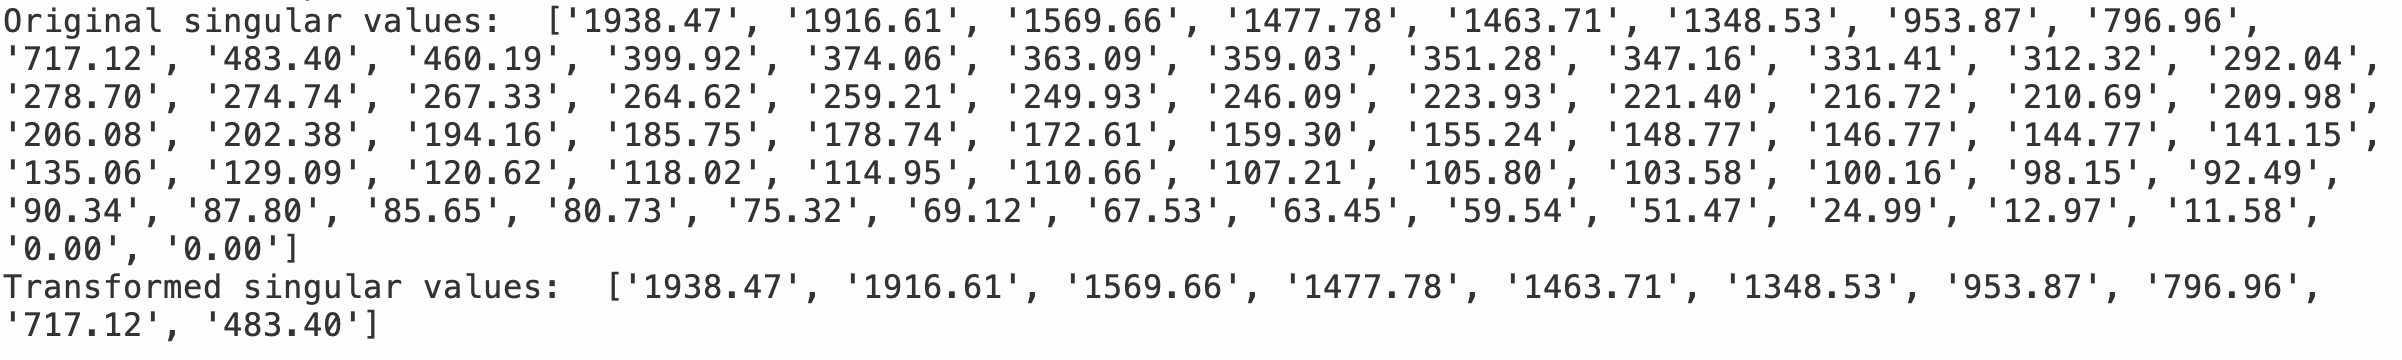
\includegraphics[width=\textwidth]{docs//assets/svd.png}
    \caption{Explained Variance Ratio - SVD}
    \label{fig:svd}
\end{figure}

\subsubsection{Variance Inflation Factor (VIF) Analysis}

\begin{table}[ht]
    \centering
    \begin{tabular}{lr}
    \toprule
    Feature & VIF \\
    \midrule
    \hline % This line adds a horizontal line between the field names and rows
    rating & 1.027474 \\
    ratingCount & 1.088795 \\
    priceInUSD & 1.003364 \\
    isAdSupported & 1.401645 \\
    isInAppPurchases & 1.503515 \\
    isEditorsChoice & 1.018758 \\
    sizeInMB & 1.180538 \\
    appAgeInDays & 1.225581 \\
    lastUpdateAgeInDays & 1.218999 \\
    \end{tabular}
    \caption{VIF of features}
    \label{tab:vif}
\end{table}
% \begin{table}[ht]
%     \centering
%     \begin{tabular}{lr}
%     \toprule
%                 Feature &      VIF \\
%     \midrule
%                  rating & 1.027474 \\
%             ratingCount & 1.088795 \\
%              priceInUSD & 1.003364 \\
%           isAdSupported & 1.401645 \\
%        isInAppPurchases & 1.503515 \\
%         isEditorsChoice & 1.018758 \\
%                sizeInMB & 1.180538 \\
%            appAgeInDays & 1.225581 \\
%     lastUpdateAgeInDays & 1.218999 \\
%     \end{tabular}
%     \caption{VIF of features}
%     \label{tab:vif}
% \end{table}


Table~\ref{tab:vif} displays the VIF for each numeric feature in the dataset. All VIF values are below 2.5, indicating an absence of collinearity within this dataset. As per various sources, a VIF greater than 5 is generally considered a cause for concern regarding collinearity.

\subsubsection{Collinearity Analysis}

The VIF analysis clearly indicates \textbf{collinearity does not exist} in this dataset. However, the application of one-hot encoding to categorical features did introduce some degree of collinearity, which also known as "Dummy Variable Trap" as revealed by the PCA. This issue can be addressed by dropping one column from each set of dummy variables.

\subsubsection{Observation on Dimensionality Reduction}

Comparing the methods used, Random Forest Analysis is notably informative, providing valuable insights into feature importance, which can not be obtained by PCA. SVD could be advantageous for datasets with images, videos or text, as it is meaningful in data compression and information extraction, though its effectiveness varies. In this dataset, the impact of SVD is less distinct due to the addition of 62 dummy variables through one-hot encoding, which are less amenable to decomposition and may contribute to multicollinearity. VIF analysis, on the other hand, is extremely useful as it precisely quantifies dataset collinearity.

Despite a longer computation time, \textbf{Random Forest Analysis} is recommended for this dataset as a better approach for feature selection rather than traditional dimensionality reduction. It provides essential information on each feature, which is highly beneficial for informed decision-making in feature selection.

\subsection{Discretization \& Binarization}
\subsubsection{Discretization of \texttt{minimumInstalls} Column}

The \texttt{Minimum Installs} feature categorizes app installations into 18 distinct groups, ranging from 0, 1, 5, 10, 50, 100, up to 5B and 10B. Utilizing this categorical feature as a target in analysis can lead to excessive complexity and a heightened risk of over-fitting due to the multitude of classes. To mitigate this issue, regrouping the installation categories proves to be a viable solution.

\subsection{One-hot Encoding of Categorical Values}

By applying \texttt{pd.get\_dummies} to the \texttt{category}, \texttt{minAndroidVersion}, and \texttt{contentRating} columns, these categorical variables are transformed into a numerical format suitable for analysis. According to the Random Forest Analysis, the most significant features include \texttt{category\_Productivity}, \texttt{category\_Social}, \texttt{minAndroidVersion\_8}, and \texttt{minAndroidVersion\_7}. Based on the combined insights from Random Forest and PCA, these selected columns are deemed crucial as they are among the top contributors to explaining at least 85\% of the dataset's variance.

\subsection{Variable Transformation}

Standardization is not necessary for decision tree and several other algorithms due to their insensitivity to data scale. In this part of the project, a new standardized dataframe is created, ensuring that the original data remains unaltered. This approach allows for the flexibility to apply different algorithms, both those that benefit from standardization and those that do not.

\subsection{Anomaly Detection}

\begin{figure}
    \centering
    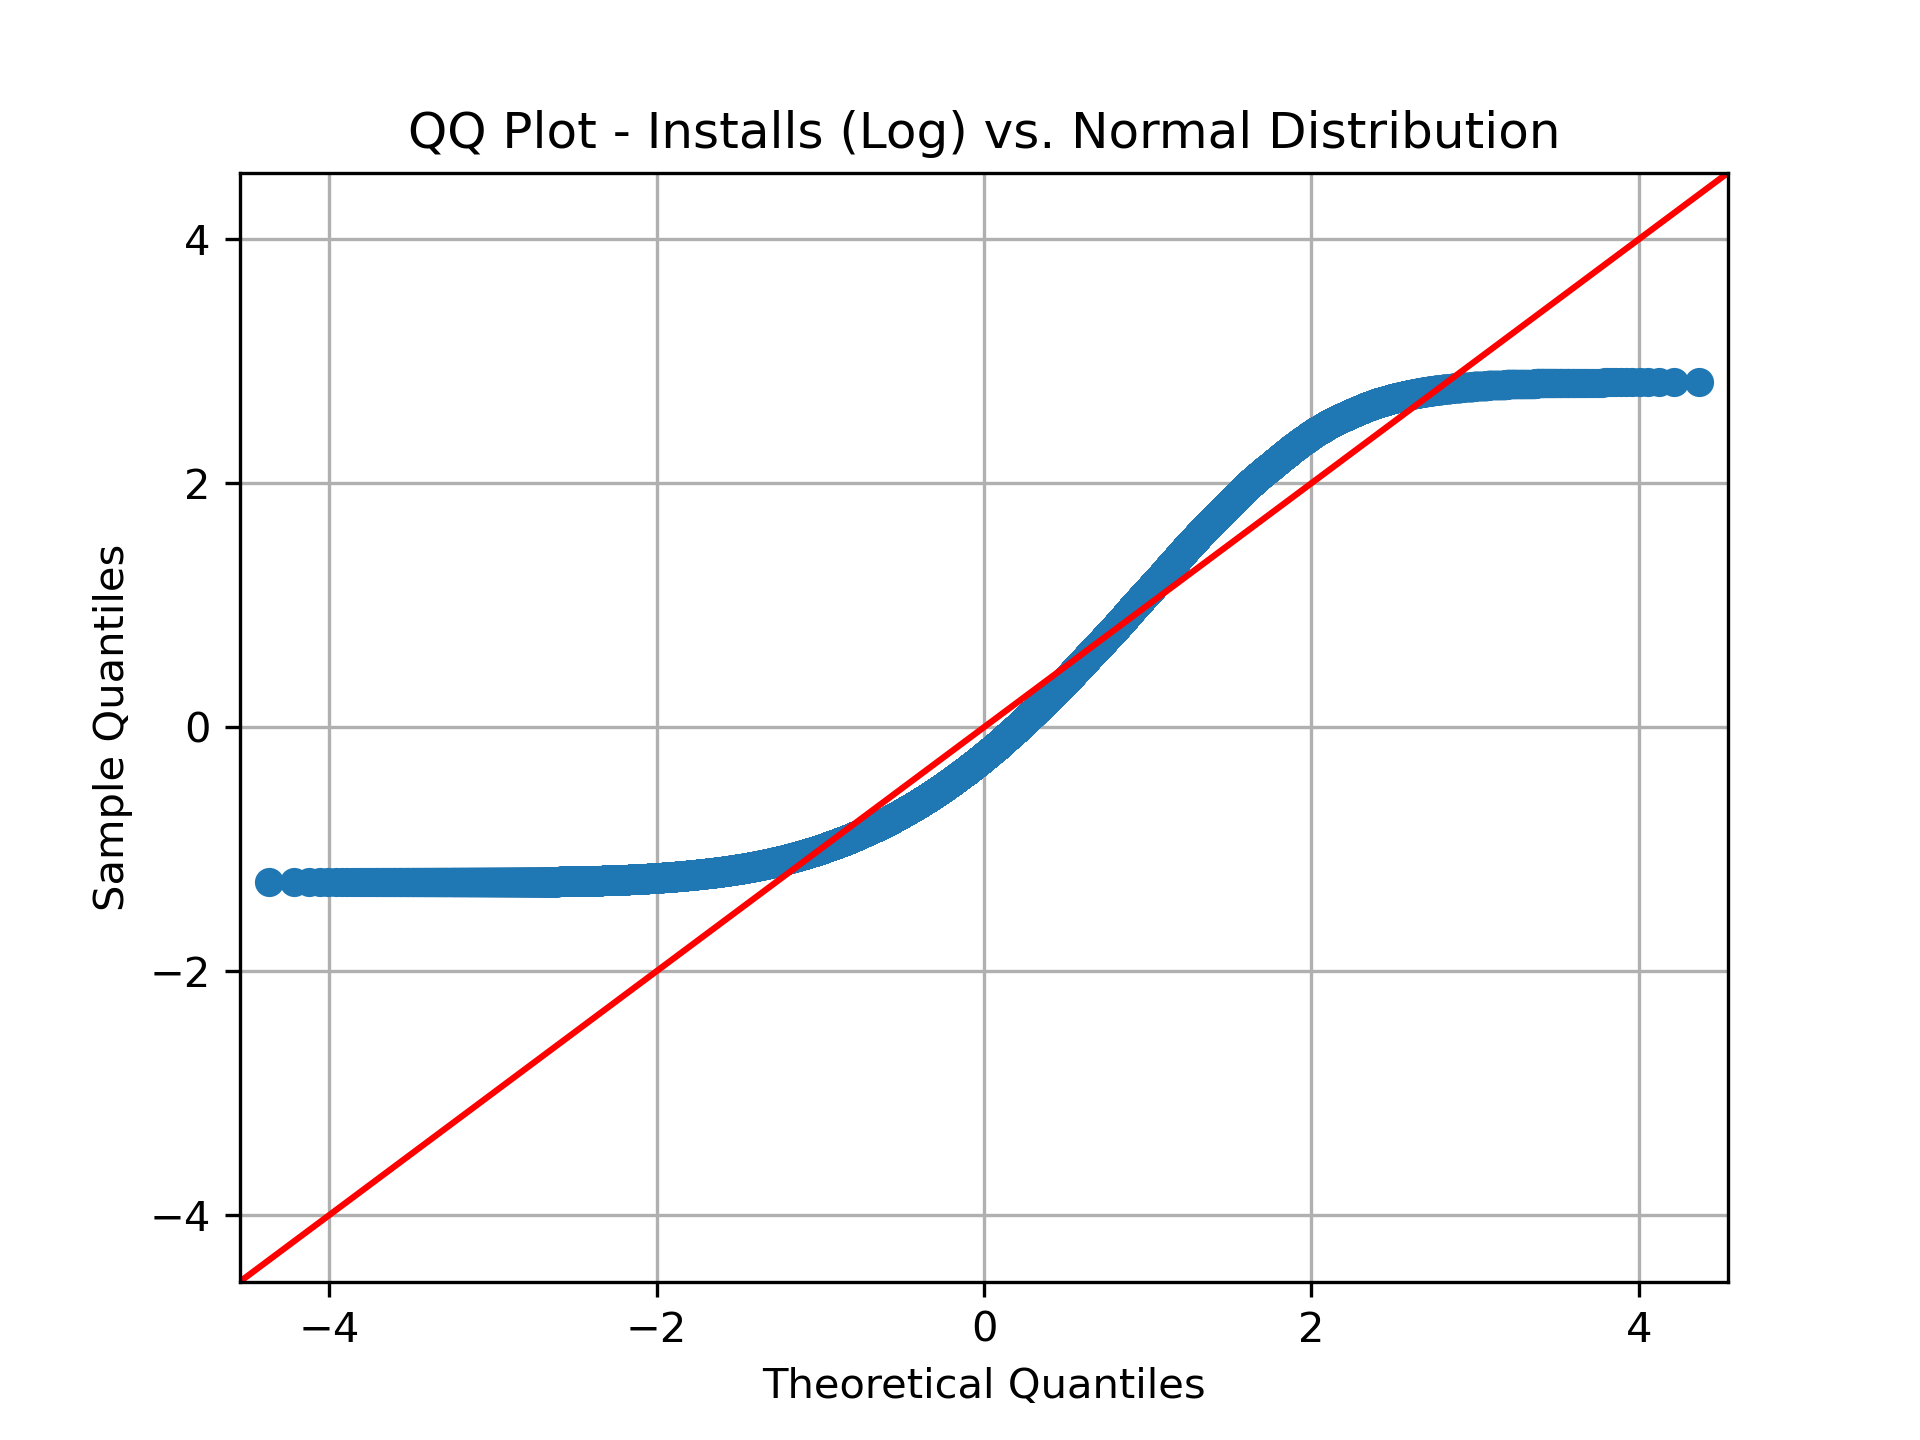
\includegraphics[width=1\linewidth]{docs//assets/qqplot.png}
    \caption{QQ Plot of Installs (Log) vs Normal Distribution}
    \label{fig:qqplot}
\end{figure}

In this part of the pre-processing, normalization tests and IQR outlier removal are utilized. The target observes no distribution at first, this issue is solved by applying \texttt{np.log10}. Unfortunately even after logarithmic transformation, the data did not pass \textbf{Shapiro test}. Figure~\ref{fig:qqplot} shows a part of observations in Installs after logarithmic transformation conforms to normal distribution 

After outlier removal using IQR method, the target still can not pass Shapiro test. In order to keep useful information, no further outlier removal is executed.



\subsection{Sample Covariance Matrix and Sample Pearson Correlation Coefficient Matrix}

\begin{figure}[h]
    \centering
    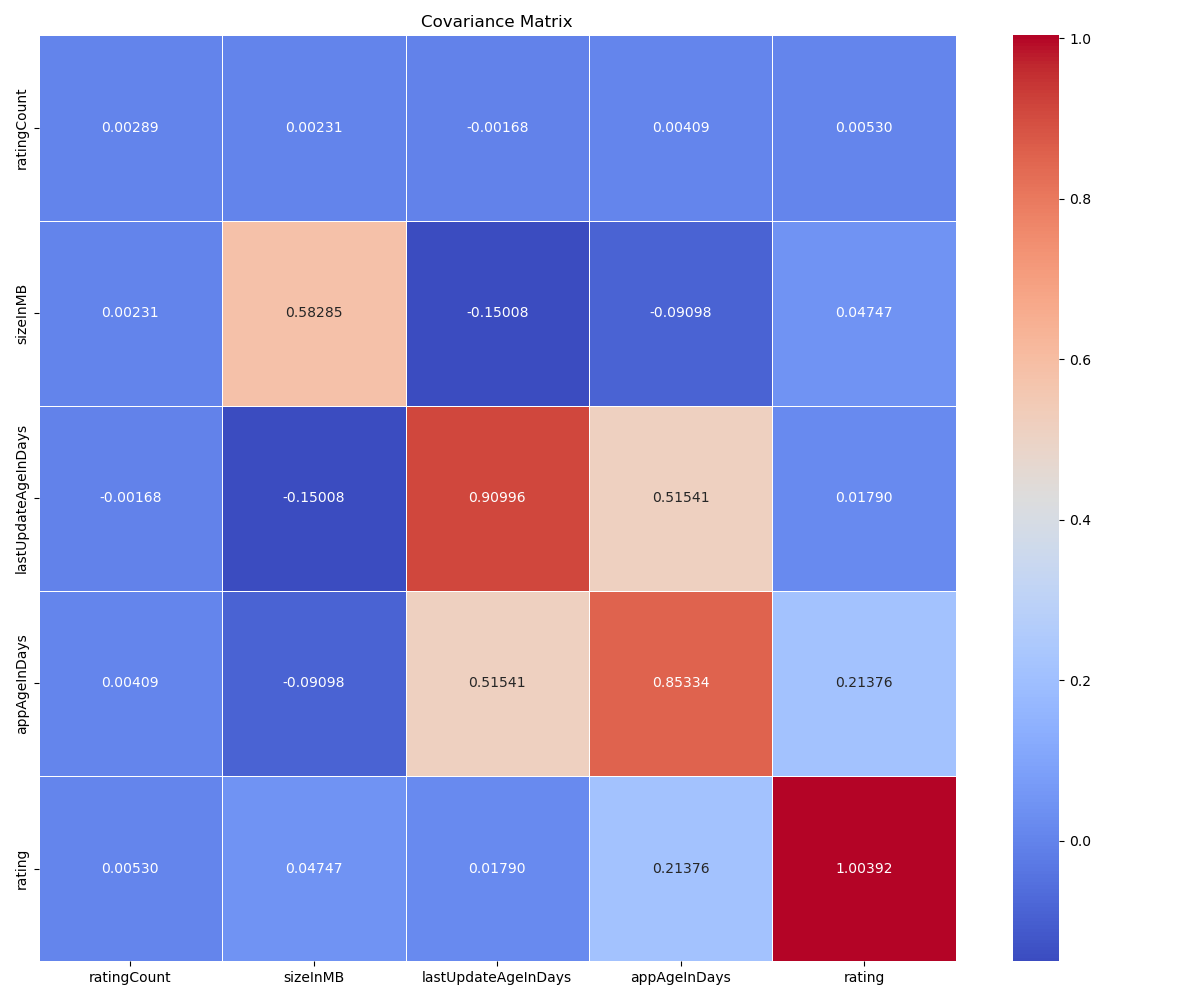
\includegraphics[width=\textwidth]{docs//assets/cov.png}
    \caption{Sample Covariance Matrix}
    \label{fig:cov}
\end{figure}

\begin{figure}[h]
    \centering
    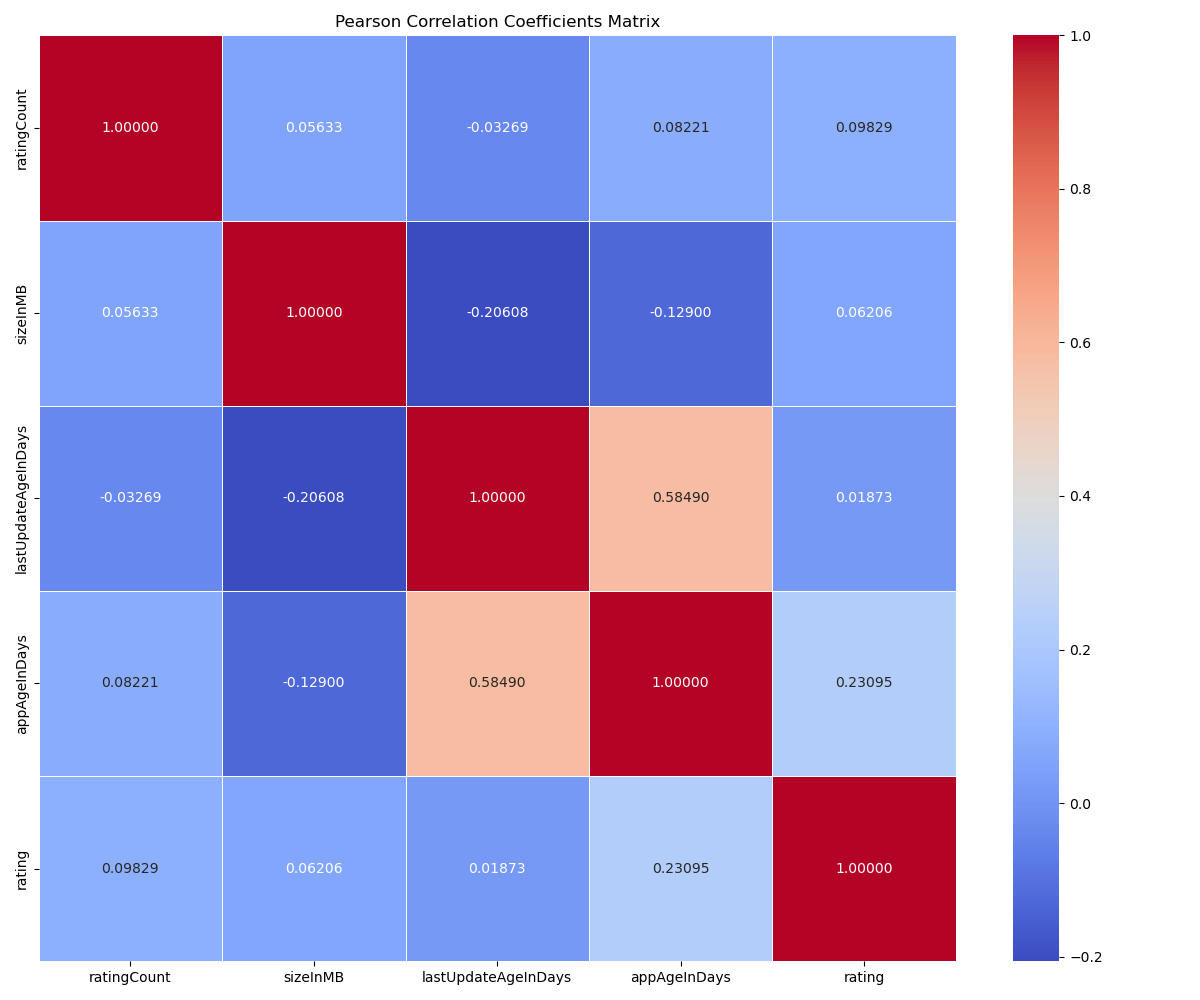
\includegraphics[width=\textwidth]{docs//assets/cor.png}
    \caption{Sample Pearson Covariance Correlation Matrix}
    \label{fig:cor}
\end{figure}

Figure~\ref{fig:cov} and Figure~\ref{fig:cor} represent the covariance matrix and the correlation matrix of the dataset, respectively. The low covariance, combined with the earlier analysis indicating a lack of collinearity among variables, is beneficial for model training. This absence of collinearity, particularly in regression models, reduces the risk of multicollinearity, leading to more stable estimates of regression coefficients

The intermediate positive correlation between \texttt{appAgeInDays} and \texttt{lastUpdateAgeInDays} (0.58) is natural. An old app does not mean it does not receive updates very often. Therefore, the higher \texttt{appAgeInDays} is, possibly but not necessarily the higher \texttt{lastUpdateAgeInDays} is.

\subsection{Balanced or Imbalanced Data}

\begin{figure}
    \centering
    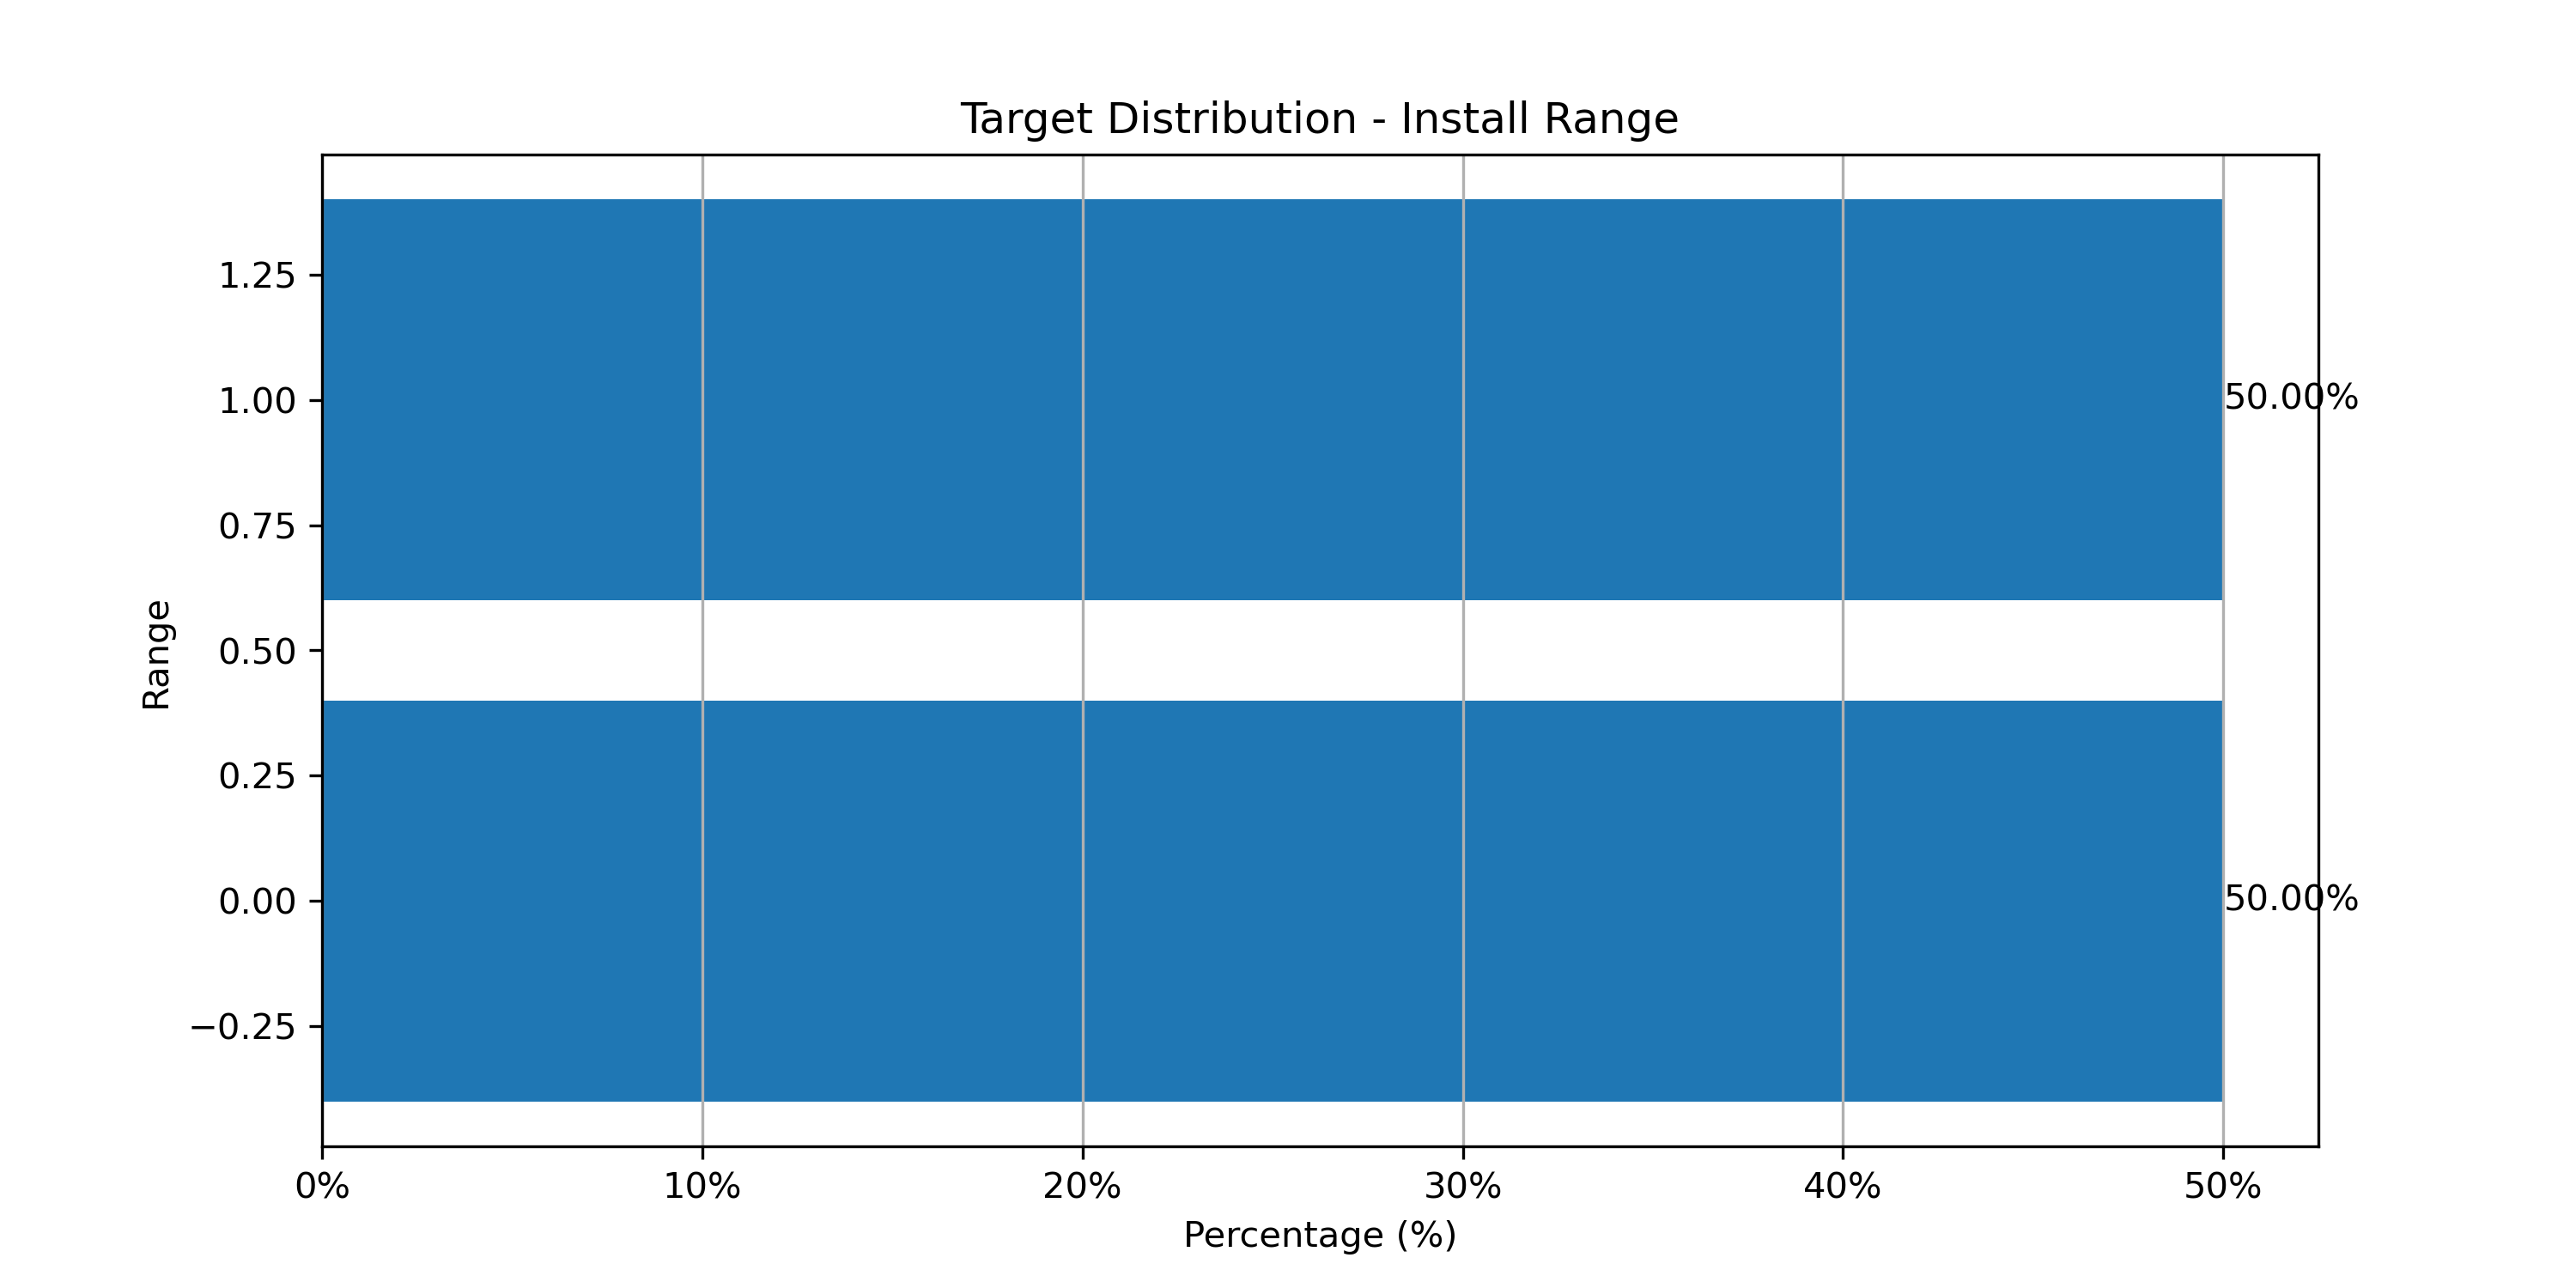
\includegraphics[width=1\linewidth]{docs//assets/target_low_high.png}
    \caption{Target Distribution after Qcut}
    \label{fig:target}
\end{figure}

In order to make sure target is balanced, \texttt{pd.qcut} is utilized. Figure~\ref{fig:target} shows the balanced target distribution after discretization and binarization.

% Rest of the document continues with similar formatting and structuring...


% \section{Phase 1}
% % Description of your dataset goes here.
% \subsection{Data Cleaning}

% \subsubsection{Raw data overview}
% This chart contains the percentage of non-applicable (N/A) data and the uniqueness of each original feature. During the forthcoming stages of analysis and data cleansing, certain unique identifiers, such as App Id, might be discarded due to their limited informative value. 'Minimum Installs' and 'Maximum Installs' represent two distinct aspects of installation counts: the former indicates a range, whereas the latter provides a precise, continuous figure. In subsequent steps, I will conduct a series of operations to evaluate the relevance of each feature, making essential modifications to optimize the data for the training process.

% \begin{figure}[h]
% \centering
% 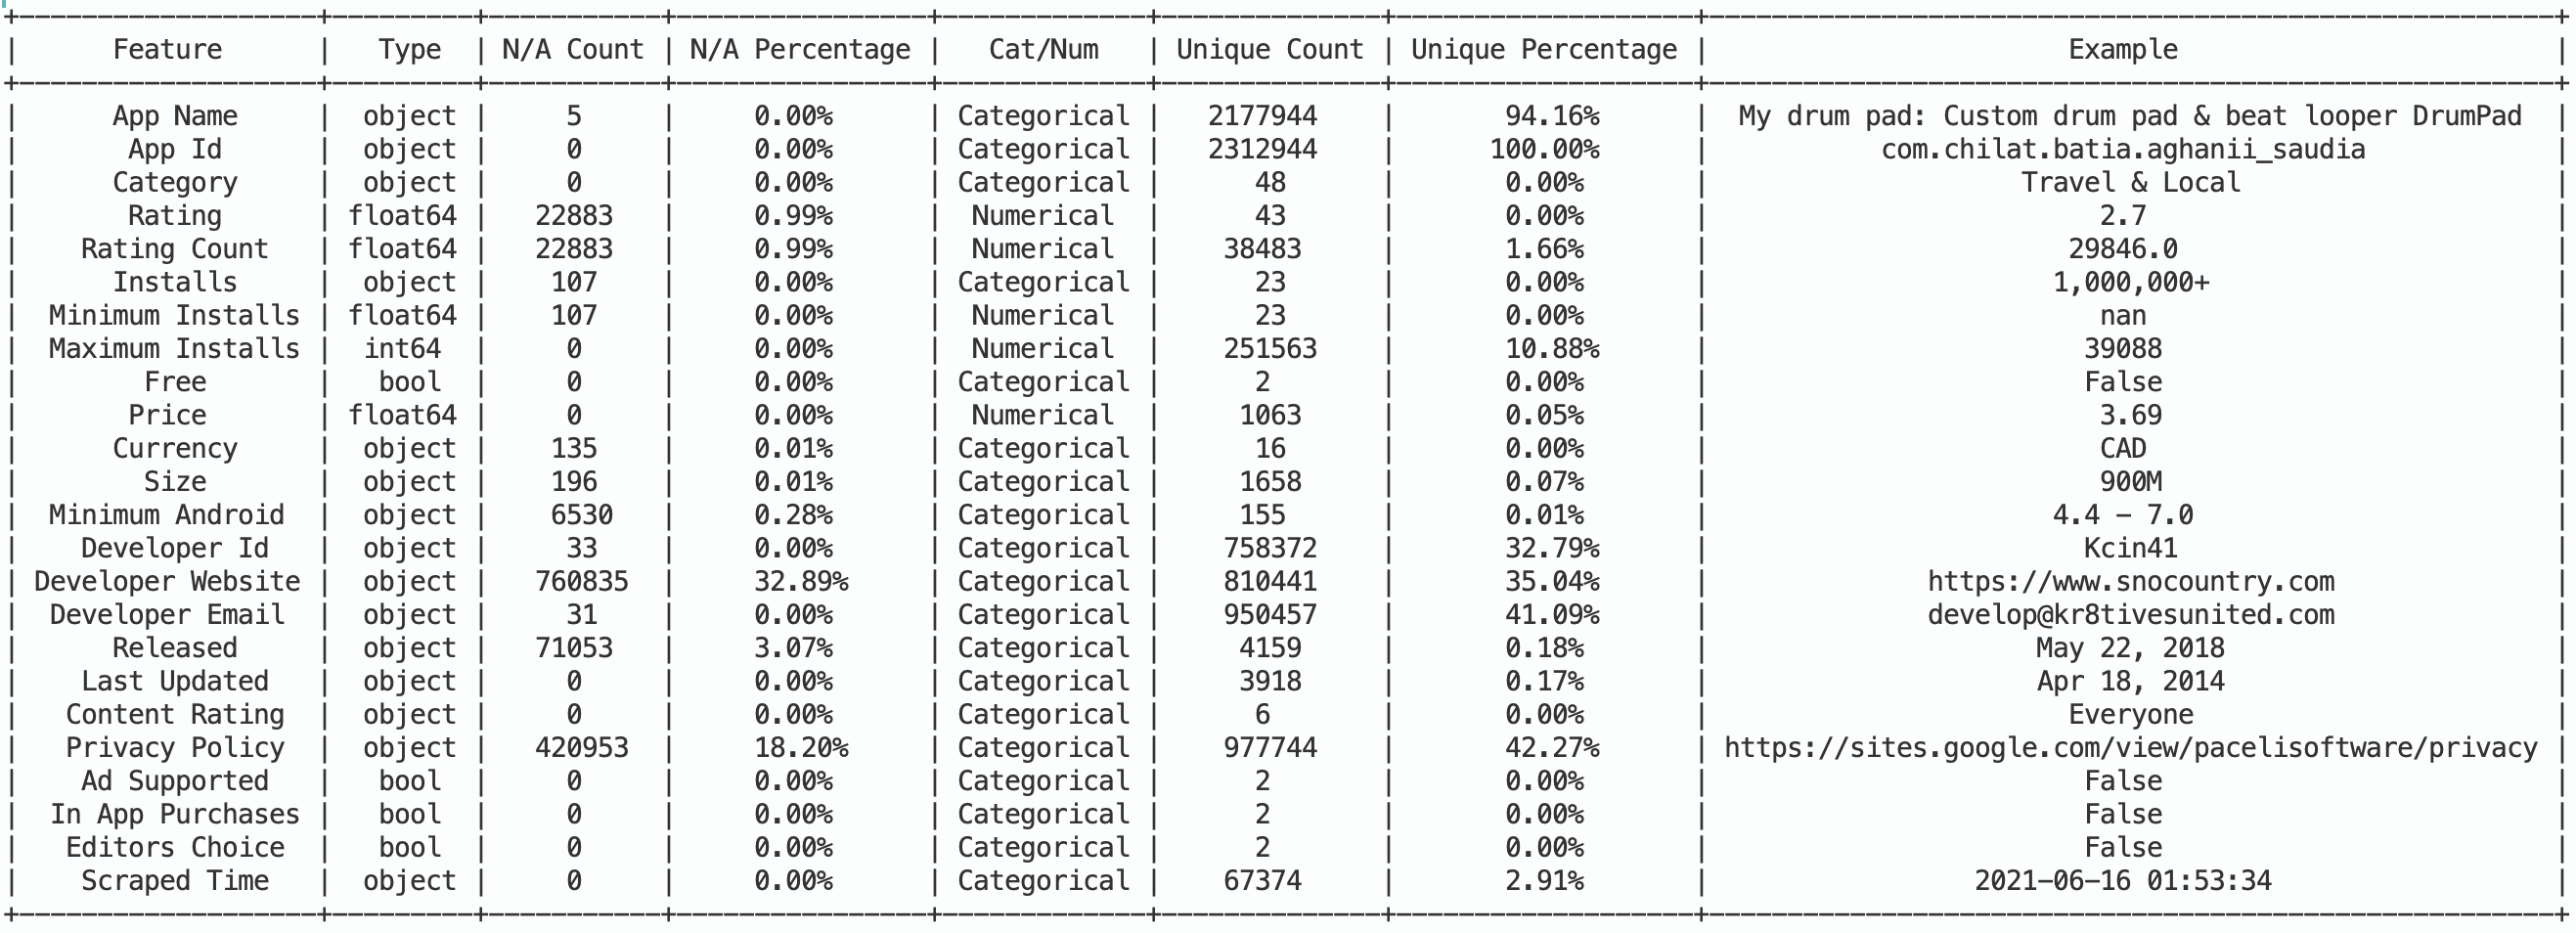
\includegraphics[width=0.8\textwidth]{docs//assets/raw-data-overview.png}
% \caption{Raw data overview}
% \end{figure}

% \subsubsection{N/A values percentage}

% \begin{figure}[h]
% \centering
% 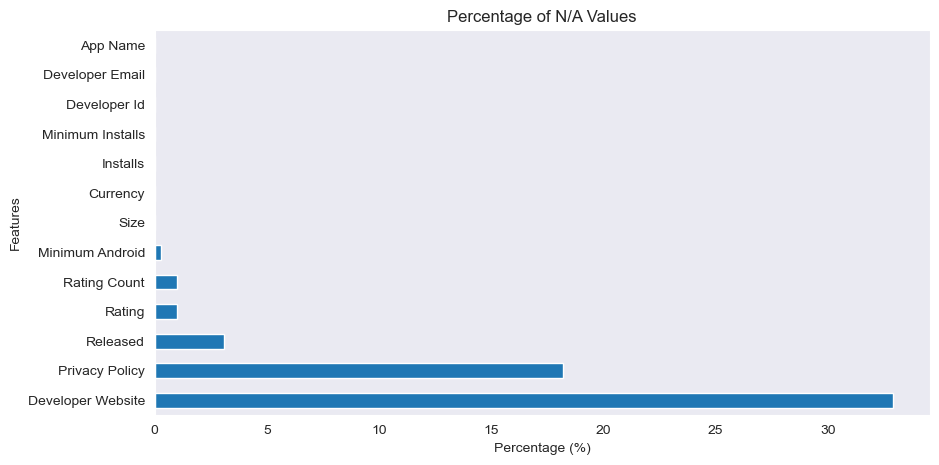
\includegraphics[width=1\textwidth]{docs//assets/percentage_na.png}
% \caption{N/A values percentage}
% \end{figure}

% For Developer Website and Privacy Policy, due to high observation of N/A values, removing the features makes more sense than removing rows with N/A values.

% \subsection{Data Duplication}

% \subsubsection{Duplication in "Currency" column}

% \begin{figure}[h]
% \centering
% 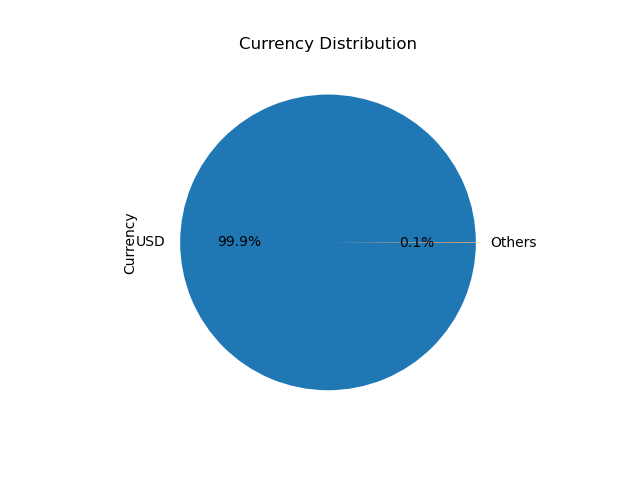
\includegraphics[width=\textwidth]{docs//assets/currency.png}
% \caption{Currency Distribution}
% \end{figure}

% In Figure X, it is evident that the "USD" currency represents over 99.9\% of the dataset. By removing observations in other currencies and subsequently deleting the "Currency" column, we can retain 99.9\% of the data while effectively reducing its dimensionality. This approach streamlines the dataset, focusing on the predominant currency for a more efficient analysis.

% \subsubsection{Duplication between "Installs" and "Minimum Installs"}

% \begin{figure}[h]
% \centering
% \includegraphics[width=\textwidth]{docs//assets/pic.png}
% \caption{Currency Distribution}
% \end{figure}

% The dataset contains three columns related to app installations, each named with variations of the word 'Installs.' Upon examination, 'Maximum Installs' is found to be a continuous numerical value, whereas 'Installs' and 'Minimum Installs' represent a range, indicating the number of app downloads. Additionally, the 'Installs' column includes characters such as '+' and ',', categorizing it as a string. The code presented in Figure X is used to determine whether the 'Installs' and 'Minimum Installs' columns are equivalent.

% \subsubsection{Duplication between "Free" and "Price"}

% Given that the price of free items is listed as 0, the 'Free' column becomes redundant and has therefore been removed from the dataset.


% \subsection{Aggregation}

% \subsubsection{Aggregation of Android versions}

% \begin{figure}[h]
% \centering
% \includegraphics[width=\textwidth]{docs//assets/pic.png}
% \caption{Currency Distribution}
% \end{figure}

% \text{The 'Minimum Android' column comprises 27 unique values, each representing a different Android version required for the app's operation. These versions are denoted as strings, such as '4.1.2'. Given that variations in minor versions do not significantly enhance the analysis of this dataset, a more effective approach involves aggregating these versions by their major numbers (e.g., 4, 5, etc.). Figure X displays a pie chart illustrating the distribution of these major Android versions after aggregation.}

% \subsection{Dimensionality Reduction}
% \subsubsection{Random Forest Analysis}
% \textbf{Steps:}
% \begin{enumerate}
%     \item \textbf{Data Preparation}
%     \begin{itemize}
%         \item Remove target variables
%         \item Convert categorical columns (category, contentRating) into dummy variables using \texttt{pd.get\_dummies}
%     \end{itemize}
%     \item \textbf{Split the data}
%     \item \textbf{Model initialization and training}
%     \item \textbf{Model prediction}
%     \item \textbf{Feature importance visualization}
% \end{enumerate} % End the enumerate environment here
% \begin{figure}[h]
% \centering
% \includegraphics[width=\textwidth]{docs//assets/pic.png}
% \caption{Currency Distribution}
% \end{figure}
% % Now the text is no longer part of the enumerate environment
% \noindent\text{The horizontal bar plot in Figure X allows us to infer that 'ratingCount' is the most significant feature, followed by 'sizeInMB', 'minAndroidVersion', 'lastUpdateAgeInDays', and 'appAgeInDays'. This insight, derived from the Random Forest Analysis, guides subsequent preprocessing steps, aiding in decisions regarding the inclusion or exclusion of specific features.}

% \subsubsection{Principle Component Analysis and Condition Number}

% \noindent\text{Figure X demonstrates that a combination of 10 features cumulatively accounts for 85\% of the variance. The dataset, transformed through PCA, consists of 68 columns, reduced from the original 71. This reduction is likely due to the application of pd.get\_dummies on three features, suggesting that PCA has effectively discarded three columns whose information is captured by the remaining data.}

% \begin{figure}[h]
% \centering
% \includegraphics[width=\textwidth]{docs//assets/pic.png}
% \caption{Currency Distribution}
% \end{figure}

% \text{The program additionally computed the condition number. Prior to the PCA transformation, the condition number was exceedingly high. However, following the transformation, it significantly reduced to 164.65. This decrease in the condition number implies that potential collinearity has been eliminated. Such collinearity might have originated from the use of the get\_dummies method.}

% \begin{figure}[h]
% \centering
% \includegraphics[width=\textwidth]{docs//assets/pic.png}
% \caption{Currency Distribution}
% \end{figure}

% \subsubsection{Singular Value Decomposition Analysis}

% \begin{figure}[h]
% \centering
% \includegraphics[width=\textwidth]{docs//assets/pic.png}
% \caption{Currency Distribution}
% \end{figure}


% \noindent\text{Following the PCA analysis, 10 features were chosen for the SVD (Singular Value Decomposition) transformation. Figure X presents a comparison of the dataset's singular values before and after the SVD transformation. It is observed that the singular values remain consistent throughout the process. The transformed dataset comprises 10 singular values, each representing the most variance in the data.}

% \subsubsection{Variance Inflation Factor (VIF) Analysis}

% \begin{figure}[h]
% \centering
% \includegraphics[width=\textwidth]{docs//assets/pic.png}
% \caption{Currency Distribution}
% \end{figure}


% \noindent\text{Figure X displays the Variance Inflation Factor (VIF) for each numeric feature in the dataset. All VIF values are below 2.5, indicating an absence of collinearity within this dataset. As per various [sources](According to different sources), a VIF greater than 5 is generally considered a cause for concern regarding collinearity.}

% \subsubsection{Collinearity Analysis}

% \noindent\text{The Variance Inflation Factor (VIF) analysis clearly indicates the absence of collinearity in this dataset. However, the application of one-hot encoding to categorical features did introduce some degree of collinearity, as revealed by the PCA. This issue can be addressed by dropping one column from each set of dummy variables.}

% \subsubsection{Observation on Dimensionality Reduction}

% \noindent\text{Comparing the methods used, Random Forest Analysis is notably informative, providing valuable insights into feature importance, an aspect not directly addressed by PCA. SVD could be advantageous for datasets with images and videos, aiding in data compression and meaningful information extraction, though its effectiveness varies. In this dataset, the impact of SVD is less distinct due to the addition of 62 dummy variables through one-hot encoding, which are less amenable to decomposition and may contribute to multicollinearity. VIF analysis, on the other hand, is extremely useful as it precisely quantifies dataset collinearity.}

% \text{Despite a longer computation time, Random Forest Analysis is recommended for this dataset as a better approach for feature selection rather than traditional dimensionality reduction. It provides essential information on each feature, which is highly beneficial for informed decision-making in feature selection.}


% \subsection{Discretization \& Binarization}
% \subsubsection{Discretization of "Minimum installs" column}
% \textbf{Steps:}

% \begin{figure}[h]
% \centering
% \includegraphics[width=\textwidth]{docs//assets/pic.png}
% \caption{Currency Distribution}
% \end{figure}
% % Now the text is no longer part of the enumerate environment
% \noindent\text{The Google Play Store categorizes app installations into 18 distinct groups, ranging from 0, 1, 5, 10, 50, 100, up to 5e9 and 1e10. Utilizing this categorical feature as a target in analysis can lead to excessive complexity and a heightened risk of overfitting due to the multitude of classes. To mitigate this issue, regrouping the installation categories proves to be a viable solution. Figure X illustrates the distribution of values in the 'installRange' after this modification. The data has been reorganized into five new, balanced groups.}


% \subsection{One-hot Encoding of Categorical Values}
% \subsubsection{Discretization of "Minimum installs" column}
% \textbf{Steps:}

% \begin{figure}[h]
% \centering
% \includegraphics[width=\textwidth]{docs//assets/pic.png}
% \caption{Currency Distribution}
% \end{figure}
% % Now the text is no longer part of the enumerate environment
% \noindent\text{By applying pd.get\_dummies to the 'category', 'minAndroidVersion', and 'contentRating' columns, these categorical variables are transformed into a numerical format suitable for analysis. According to the Random Forest Analysis, the most significant features include 'category\_Productivity', 'category\_Social', 'minAndroidVersion\_8', and 'minAndroidVersion\_7'.  Based on the combined insights from Random Forest and PCA, these selected columns are deemed crucial as they are among the top contributors to explaining at least 85\% of the dataset's variance.}

% \subsection{Variable Transformation}
% \noindent\text{Standardization is a process that normalizes the scale of data, which can enhance the performance of various algorithms. However, it's not necessary. For instance, decision tree algorithms, including their variants, do not require standardization due to their insensitivity to data scale. In this analysis, a new standardized dataframe is created, ensuring that the original data remains unaltered. This approach allows for the flexibility to apply different algorithms, both those that benefit from standardization and those that do not.}

% \subsection{Anomaly Detection}
% \begin{figure}[h]
% \centering
% \includegraphics[width=\textwidth]{docs//assets/pic.png}
% \caption{Currency Distribution}
% \end{figure}
% \noindent\text{In this analysis, the Mahalanobis distance, in conjunction with the chi-squared distribution, is utilized to identify outliers in the dataset. It's important to note that the squared Mahalanobis Distance adheres to a Chi-Square distribution. The degrees of freedom for the chi-squared test are set at 11, accounting for 10 variables and one target in the dataset. A significance level of 0.1 is chosen for outlier detection, which is a common practice in statistical analysis to balance between sensitivity and specificity in identifying outliers. Consequently, this approach led to the identification and proposed removal of approximately 235,840 observations, equating to roughly 10.8\% of the data, as outliers.}

% \subsection{Sample Covariance Matrix and Sample Pearson Correlation Coefficient Matrix}
% \begin{figure}[h]
% \centering
% \includegraphics[width=\textwidth]{docs//assets/pic.png}
% \caption{Currency Distribution}
% \end{figure}

% \text{Figure X and Figure Y represent the covariance matrix and the correlation matrix of the dataset, respectively. The low covariance, combined with the earlier analysis indicating a lack of collinearity among variables, is beneficial for model training. This absence of collinearity, particularly in regression models, reduces the risk of multicollinearity, leading to more stable estimates of regression coefficients}

% \subsection{Balanced or Imbalanced Data}
% \begin{figure}[h]
% \centering
% \includegraphics[width=\textwidth]{docs//assets/pic.png}
% \caption{Currency Distribution}
% \end{figure}

% \text{The distribution of targets depicted in Figure X indicates a balanced composition, with no single group dominating the target dataset.}


\section{Phase 2 - Regression Analysis}

\subsection{Backward Step-wise Analysis}


\begin{center}
\begin{table}
\small
\begin{tabular}{lclc}
\toprule
\textbf{Dep. Variable:}    &   installCount   & \textbf{  R-squared:         } &      0.368   \\
\textbf{Model:}            &       OLS        & \textbf{  Adj. R-squared:    } &      0.368   \\
\textbf{Method:}           &  Least Squares   & \textbf{  F-statistic:       } &      7478.   \\
\textbf{Date:}             & Thu, 07 Dec 2023 & \textbf{  Prob (F-statistic):} &      0.00    \\
\textbf{Time:}             &     20:25:58     & \textbf{  Log-Likelihood:    } & -1.5240e+05  \\
\textbf{No. Observations:} &      128408      & \textbf{  AIC:               } &  3.048e+05   \\
\textbf{Df Residuals:}     &      128397      & \textbf{  BIC:               } &  3.049e+05   \\
\textbf{Df Model:}         &          10      & \textbf{                     } &              \\
\textbf{Covariance Type:}  &    nonrobust     & \textbf{                     } &              \\
\bottomrule
\end{tabular}
%\caption{OLS Regression Results}
\begin{tabular}{lcccccc}
\toprule
                                & \textbf{coef} & \textbf{std err} & \textbf{t} & \textbf{P$> |$t$|$} & \textbf{[0.025} & \textbf{0.975]}  \\
\midrule
\textbf{const}                  &      -0.0401  &        0.003     &   -14.803  &         0.000        &       -0.045    &       -0.035     \\
\textbf{ratingCount}            &       0.5932  &        0.002     &   247.019  &         0.000        &        0.588    &        0.598     \\
\textbf{sizeInMB}               &       0.0299  &        0.002     &    12.388  &         0.000        &        0.025    &        0.035     \\
\textbf{lastUpdateAgeInDays}    &      -0.0737  &        0.002     &   -30.092  &         0.000        &       -0.079    &       -0.069     \\
\textbf{minAndroidVersion\_8}   &      -0.0554  &        0.034     &    -1.616  &         0.106        &       -0.123    &        0.012     \\
\textbf{appAgeInDays}           &       0.0703  &        0.002     &    28.737  &         0.000        &        0.065    &        0.075     \\
\textbf{rating}                 &      -0.0119  &        0.002     &    -5.293  &         0.000        &       -0.016    &       -0.007     \\
\textbf{category\_Productivity} &      -0.0101  &        0.014     &    -0.708  &         0.479        &       -0.038    &        0.018     \\
\textbf{category\_Social}       &      -0.0320  &        0.016     &    -1.957  &         0.050        &       -0.064    &     4.45e-05     \\
\textbf{isInAppPurchases}       &       0.1569  &        0.005     &    30.024  &         0.000        &        0.147    &        0.167     \\
\textbf{minAndroidVersion\_7}   &      -0.1098  &        0.020     &    -5.508  &         0.000        &       -0.149    &       -0.071     \\
\bottomrule
\end{tabular}
\caption{OLS Summary of All Features}
\label{tab:ols-1}
\end{table}
\end{center}


This part of project uses \texttt{statsmodel.OLS} model to estimate a multiple linear regression model. The dependent variable for this model is installCount. Table~\ref{tab:ols-1} is the summary of the first fit for this linear model. From $R^2$, it's clear that the model does not produce a good fit. Further inspection on features is needed. 

Utilizing backward step-wise analysis, \texttt{category\_Productivity} is the first one to remove.\textit{ A small p-value indicates that it is unlikely to observe such a substantial association between the predictor and the response due to chance, in the absence of any real association between the predictor and the response. Hence, if we see a small p-value, then we can infer that there is an association between the predictor and the response}\cite{james2023introduction}. Student's t-tests on each feature's coefficient to the dependent variable are implemented by the model to determine if they significantly contribute to the model. The null hypothesis for each t-test is that the coefficient is equal to zero, meaning it has no effect. Backward step-wise regression requires the operator to remove the feature with the highest p-value until no feature observes p-value that is higher than the significance value. A drawback of this method is that the process is manual. Although I tried to automate the process into a pipeline, the encapsulated library prevented me from doing so.

\begin{center}
    \begin{table}[]
        \centering
        \scriptsize
            \begin{tabular}{cccccccc}
                \hline
                 Removed Feature & p-value & AIC & BIC & $R^2$ & Adj $R^2$ & MSE \\
                \hline
                N/A & N/A & 304816.425 & 304923.818 & 0.368 & 0.368 & 4700.899 \\
                category\_Productivity & 0.479 & 304814.926 & 304912.556 & 0.368 & 0.368 & 5223.186 \\
                minAndroidVersion\_8 & 0.105 & 304815.559 & 304903.426 & 0.368 & 0.368 & 5875.877 \\
                category\_Social & 0.052 & 304817.321 & 304895.425 & 0.368 & 0.368 & 6714.950 \\
                \hline
            \end{tabular}
        \caption{Backward Stepwise Analysis}
        \label{tab:backwise}
    \end{table}
\end{center}

Table~\ref{tab:backwise} shows the procedure of backward step-wise analysis. Although the associated features are removed, the model does not observe a higher $R^2$ value. Table~\ref{tab:ols-2} shows the OLS summary of the model after removing features with low associations. Although F-statistics is relatively high, the probability of F-Statistics is 0, which means it fails to reject the hypothesis. Also, the MSE is getting higher after removing redundant features, which is a sign of bad fit.

Considering backward step-wise analysis did not receive positive outcome for this dataset, more regressors need to be considered, for example, random forest regressor. 

\begin{table}
    \centering
    \small
    \begin{center}
        \begin{tabular}{lclc}
        \toprule
        \textbf{Dep. Variable:}       &   installCount   & \textbf{  R-squared:         } &      0.368   \\
        \textbf{Model:}               &       OLS        & \textbf{  Adj. R-squared:    } &      0.368   \\
        \textbf{Method:}              &  Least Squares   & \textbf{  F-statistic:       } &  1.068e+04   \\
        \textbf{Date:}                & Thu, 07 Dec 2023 & \textbf{  Prob (F-statistic):} &      0.00    \\
        \textbf{Time:}                &     21:35:19     & \textbf{  Log-Likelihood:    } & -1.5240e+05  \\
        \textbf{No. Observations:}    &      128408      & \textbf{  AIC:               } &  3.048e+05   \\
        \textbf{Df Residuals:}        &      128400      & \textbf{  BIC:               } &  3.049e+05   \\
        \textbf{Df Model:}            &           7      & \textbf{                     } &              \\
        \textbf{Covariance Type:}     &    nonrobust     & \textbf{                     } &              \\
        \bottomrule
        \end{tabular}
        \begin{tabular}{lcccccc}
                                      & \textbf{coef} & \textbf{std err} & \textbf{t} & \textbf{P$> |$t$|$} & \textbf{[0.025} & \textbf{0.975]}  \\
        \midrule
        \textbf{const}                &      -0.0412  &        0.003     &   -15.422  &         0.000        &       -0.046    &       -0.036     \\
        \textbf{ratingCount}          &       0.5932  &        0.002     &   247.041  &         0.000        &        0.588    &        0.598     \\
        \textbf{sizeInMB}             &       0.0299  &        0.002     &    12.429  &         0.000        &        0.025    &        0.035     \\
        \textbf{lastUpdateAgeInDays}  &      -0.0734  &        0.002     &   -30.001  &         0.000        &       -0.078    &       -0.069     \\
        \textbf{appAgeInDays}         &       0.0702  &        0.002     &    28.752  &         0.000        &        0.065    &        0.075     \\
        \textbf{rating}               &      -0.0118  &        0.002     &    -5.237  &         0.000        &       -0.016    &       -0.007     \\
        \textbf{isInAppPurchases}     &       0.1568  &        0.005     &    30.019  &         0.000        &        0.147    &        0.167     \\
        \textbf{minAndroidVersion\_7} &      -0.1097  &        0.020     &    -5.503  &         0.000        &       -0.149    &       -0.071     \\
        \bottomrule
        \end{tabular}
        \end{center}
        \begin{tabular}{lclc}
        \textbf{Omnibus:}       & 73565.243 & \textbf{  Durbin-Watson:     } &      1.995   \\
        \textbf{Prob(Omnibus):} &    0.000  & \textbf{  Jarque-Bera (JB):  } & 2705960.736  \\
        \textbf{Skew:}          &    2.156  & \textbf{  Prob(JB):          } &       0.00   \\
        \textbf{Kurtosis:}      &   25.072  & \textbf{  Cond. No.          } &       11.3   \\
        \bottomrule
        \end{tabular}
        %\caption{OLS Regression Results}
        
    \caption{OLS Summary of Remaining Features}
    \label{tab:ols-2}
\end{table}

\subsection{Random Forest Regressor}

Random forest regressor is used for a better outcome than linear regression. To begin with, a initial training of the \texttt{RandomForestRegressor} is executed. From the initial training, the feature importance can be obtained.

Figure~\ref{fig:rfg} shows the feature importances of the initial run. For all 13 features used in initial build, after the $6^{th}$ feature, importances plumbed. Therefore keeping only the features whose importance is higher than 0.05. 

\begin{figure}
    \centering
    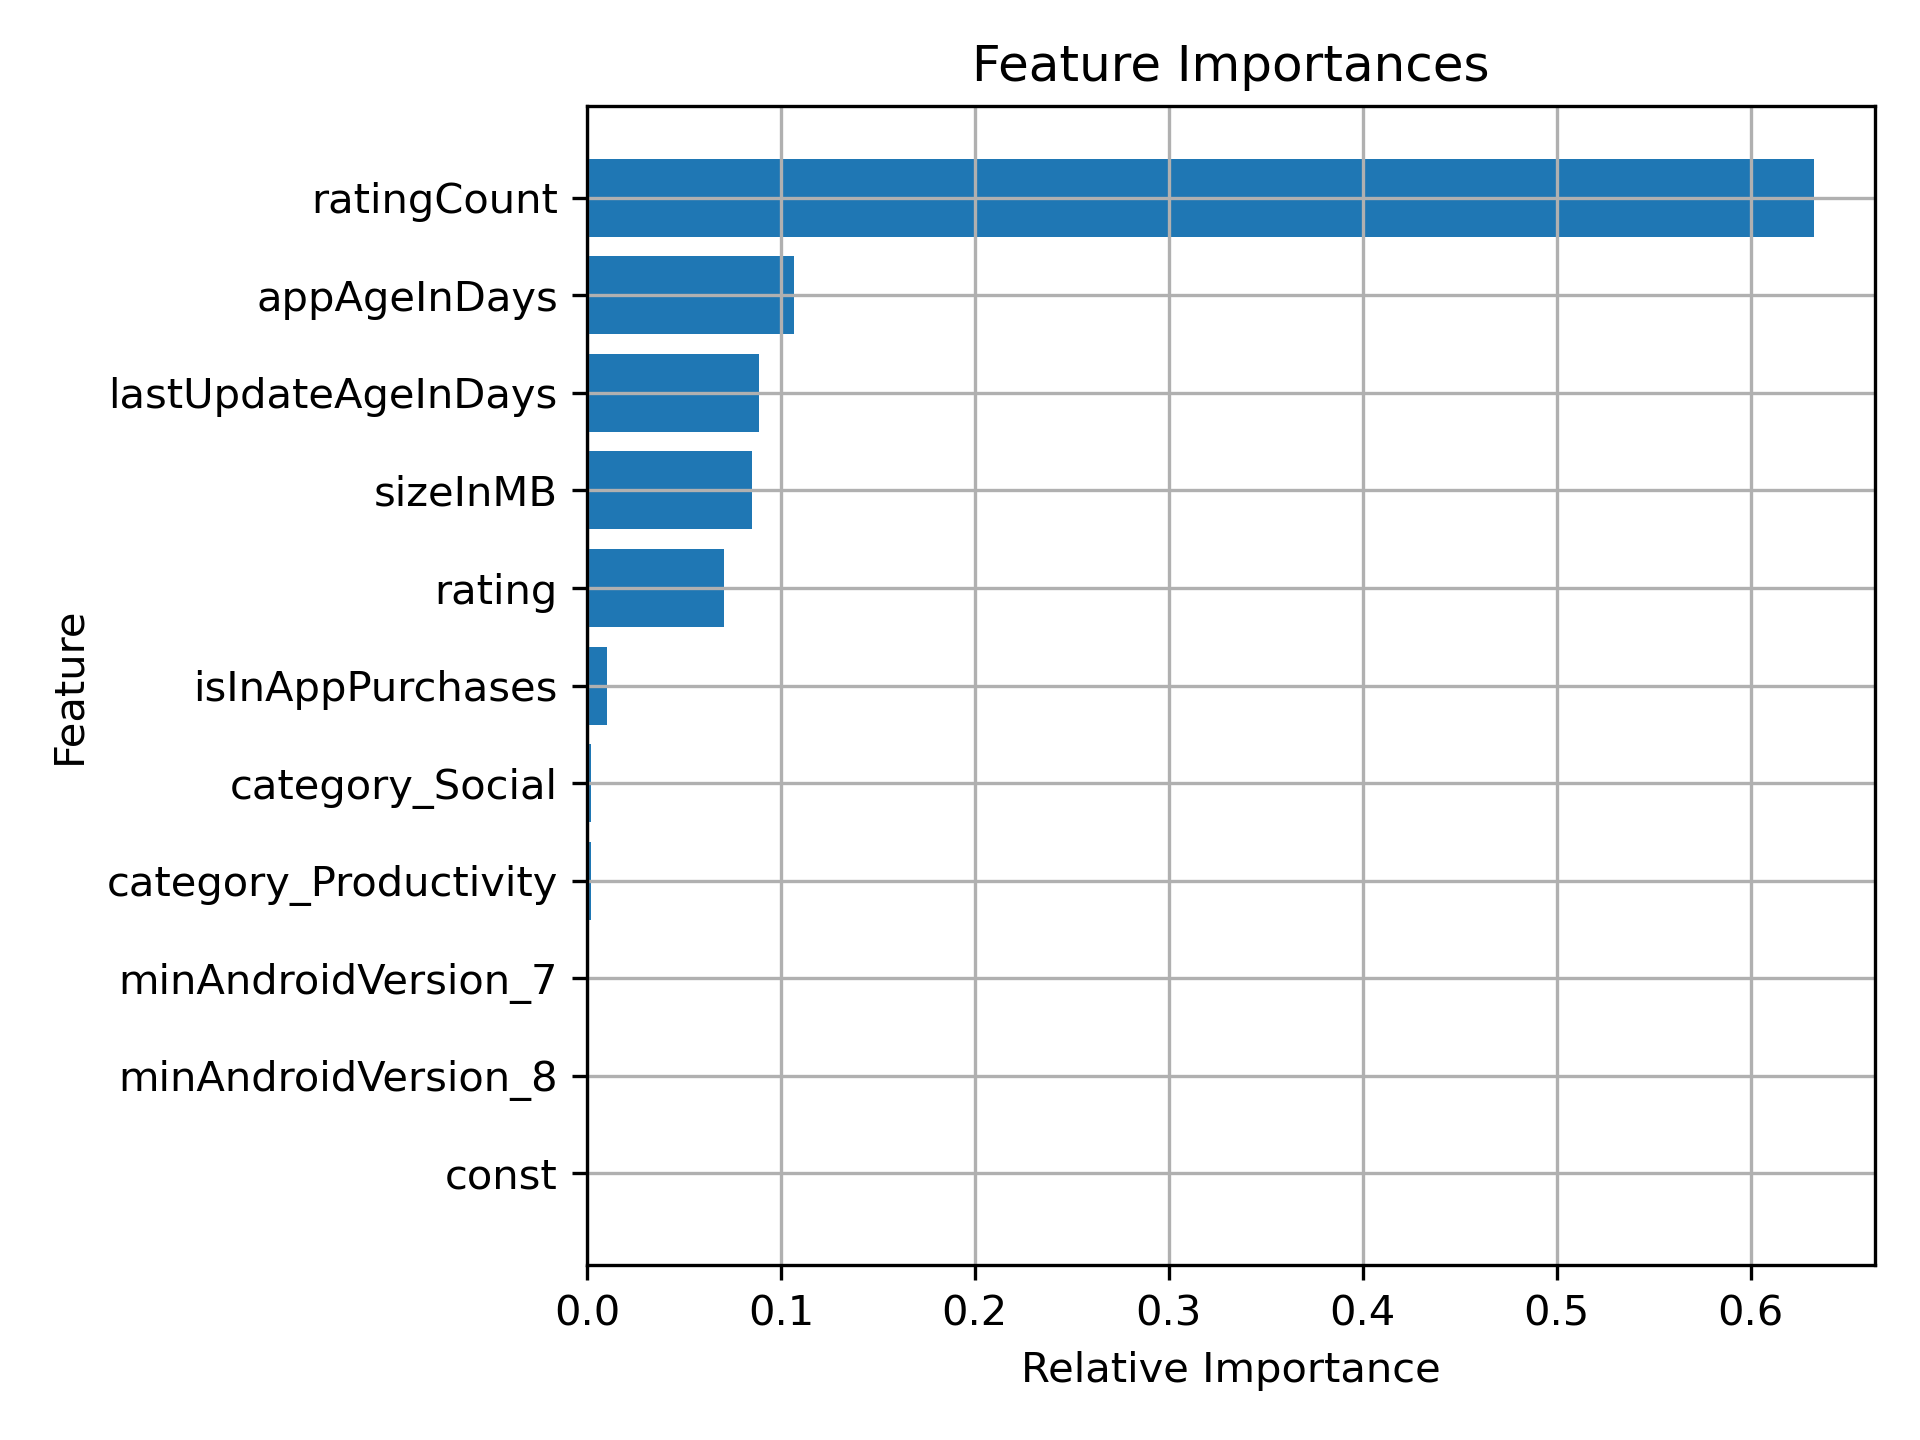
\includegraphics[width=1\linewidth]{docs//assets/regressor_feature_importances.png}
    \caption{Random Forest Regressor - Feature Importance}
    \label{fig:rfg}
\end{figure}

After setting threshold as 0.05, another training of the regressor based on the new feature matrix with only important features is executed. In order to prevent over-fitting, K-Fold cross-validation (10 folds) is used to evaluate the model, calculating MSE for each fold.

\begin{table}[h]
\centering
\scriptsize
\begin{tabular}{|c|c|c|c|c|c|c|c|c|c|c|}
\hline
\textbf{Fold 1} & \textbf{Fold 2} & \textbf{Fold 3} & \textbf{Fold 4} & \textbf{Fold 5} & \textbf{Fold 6} & \textbf{Fold 7} & \textbf{Fold 8} & \textbf{Fold 9} & \textbf{Fold 10} \\
\hline
0.42 & 0.42 & 0.41 & 0.44 & 0.43 & 0.46 & 0.42 & 0.42 & 0.44 & 0.40 \\
\hline
\end{tabular}
\caption{10-fold Cross Validation Mean Squared Error Scores}
\label{tab:kfold_scores}
\end{table}

The final result of the random forest regressor is in table~\ref{tab:rfg-results}, compared to the results in table~\ref{tab:ols-2}, the $R^{2}$ is significantly increased, meaning that this tree-based model is a better fit for this dataset. Seemingly unusual negative AIC and BIC values are also accepted\cite{burnham2003model}, and provides an apparently better fit than linear regression model. Low AIC and BIC indicates a preferred model. As observed from both table~\ref{tab:kfold_scores} and table~\ref{tab:rfg-results}, the MSE is very low. K-fold prevents possible over-fitting, that's the reason testing MSE in the table is similar to training data.



\begin{table}[ht]
\centering
\begin{tabular}{|l|l|l|l|l|}
\hline
$R^2$ & Adj $R^2$ & AIC       & BIC       & MSE  \\ \hline
0.58  & 0.58   & -27065.07 & -27023.19 & 0.43 \\ \hline
\end{tabular}
\caption{Final Regression Model Results}
\label{tab:rfg-results}
\end{table}

\begin{figure}
    \centering
    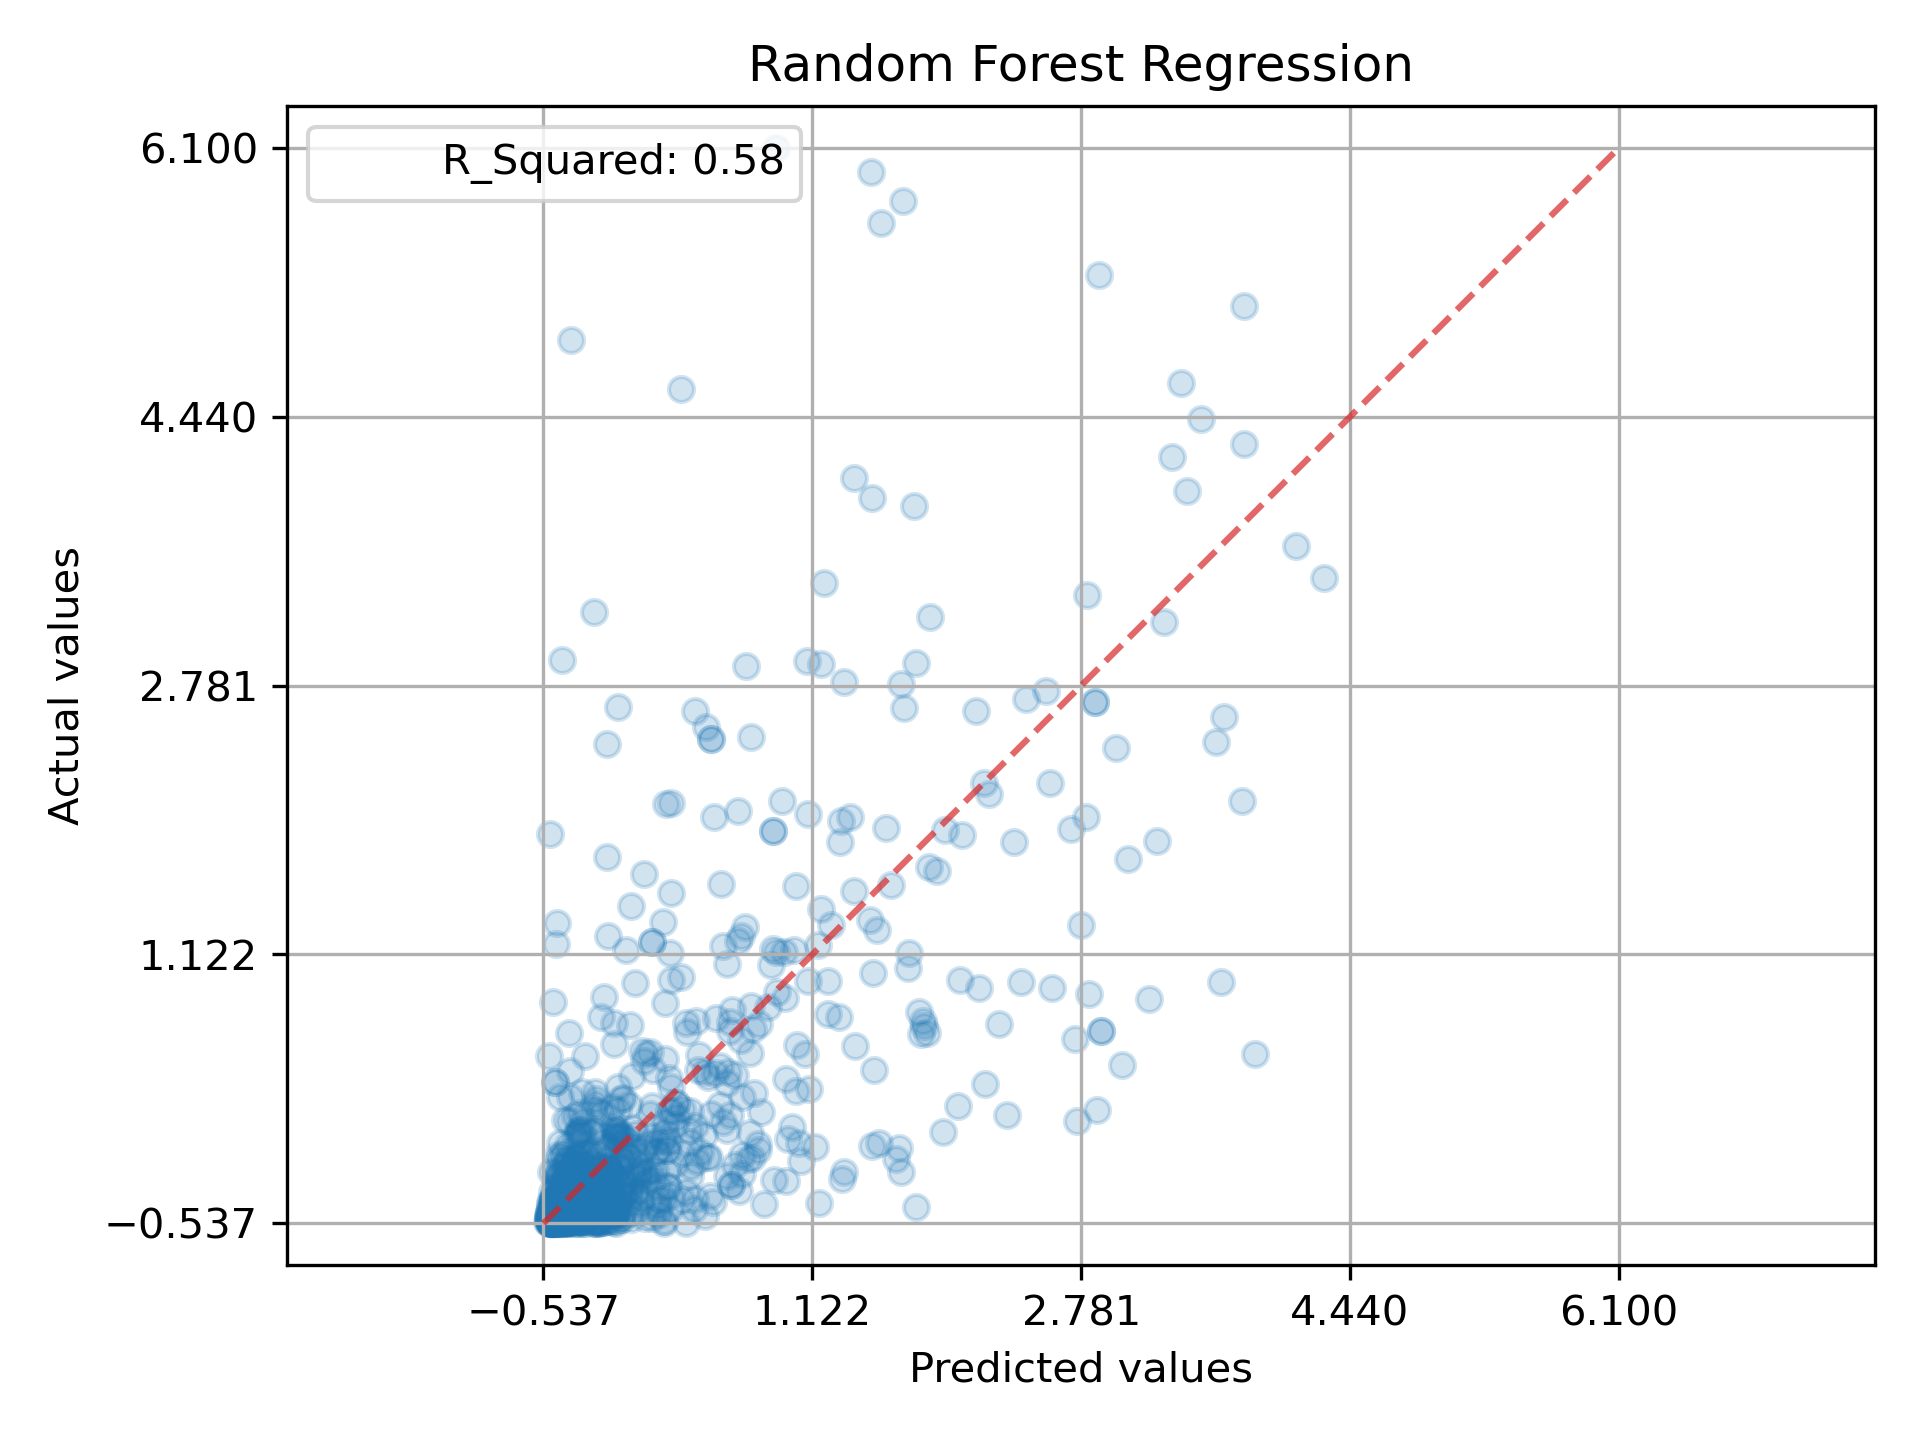
\includegraphics[width=1\linewidth]{docs//assets/regressor_prediction_error.png}
    \caption{Actual vs Predicted Values - Random Forest Regressor}
    \label{fig:rfg-scatter}
\end{figure}

Figure~\ref{fig:rfg-scatter} shows the plot of actual and predicted values via random forest regressor. Although scattered and radiactive, a better fit than linear regression is observed. Figure~\ref{fig:rfg-ci} shows the first 100 samples' predicted \texttt{installCount} and actual \texttt{installCount}. Most of values are with the boundaries of confidence interval, which indicates a good fit by the random forest regression model.

\begin{figure}
    \centering
    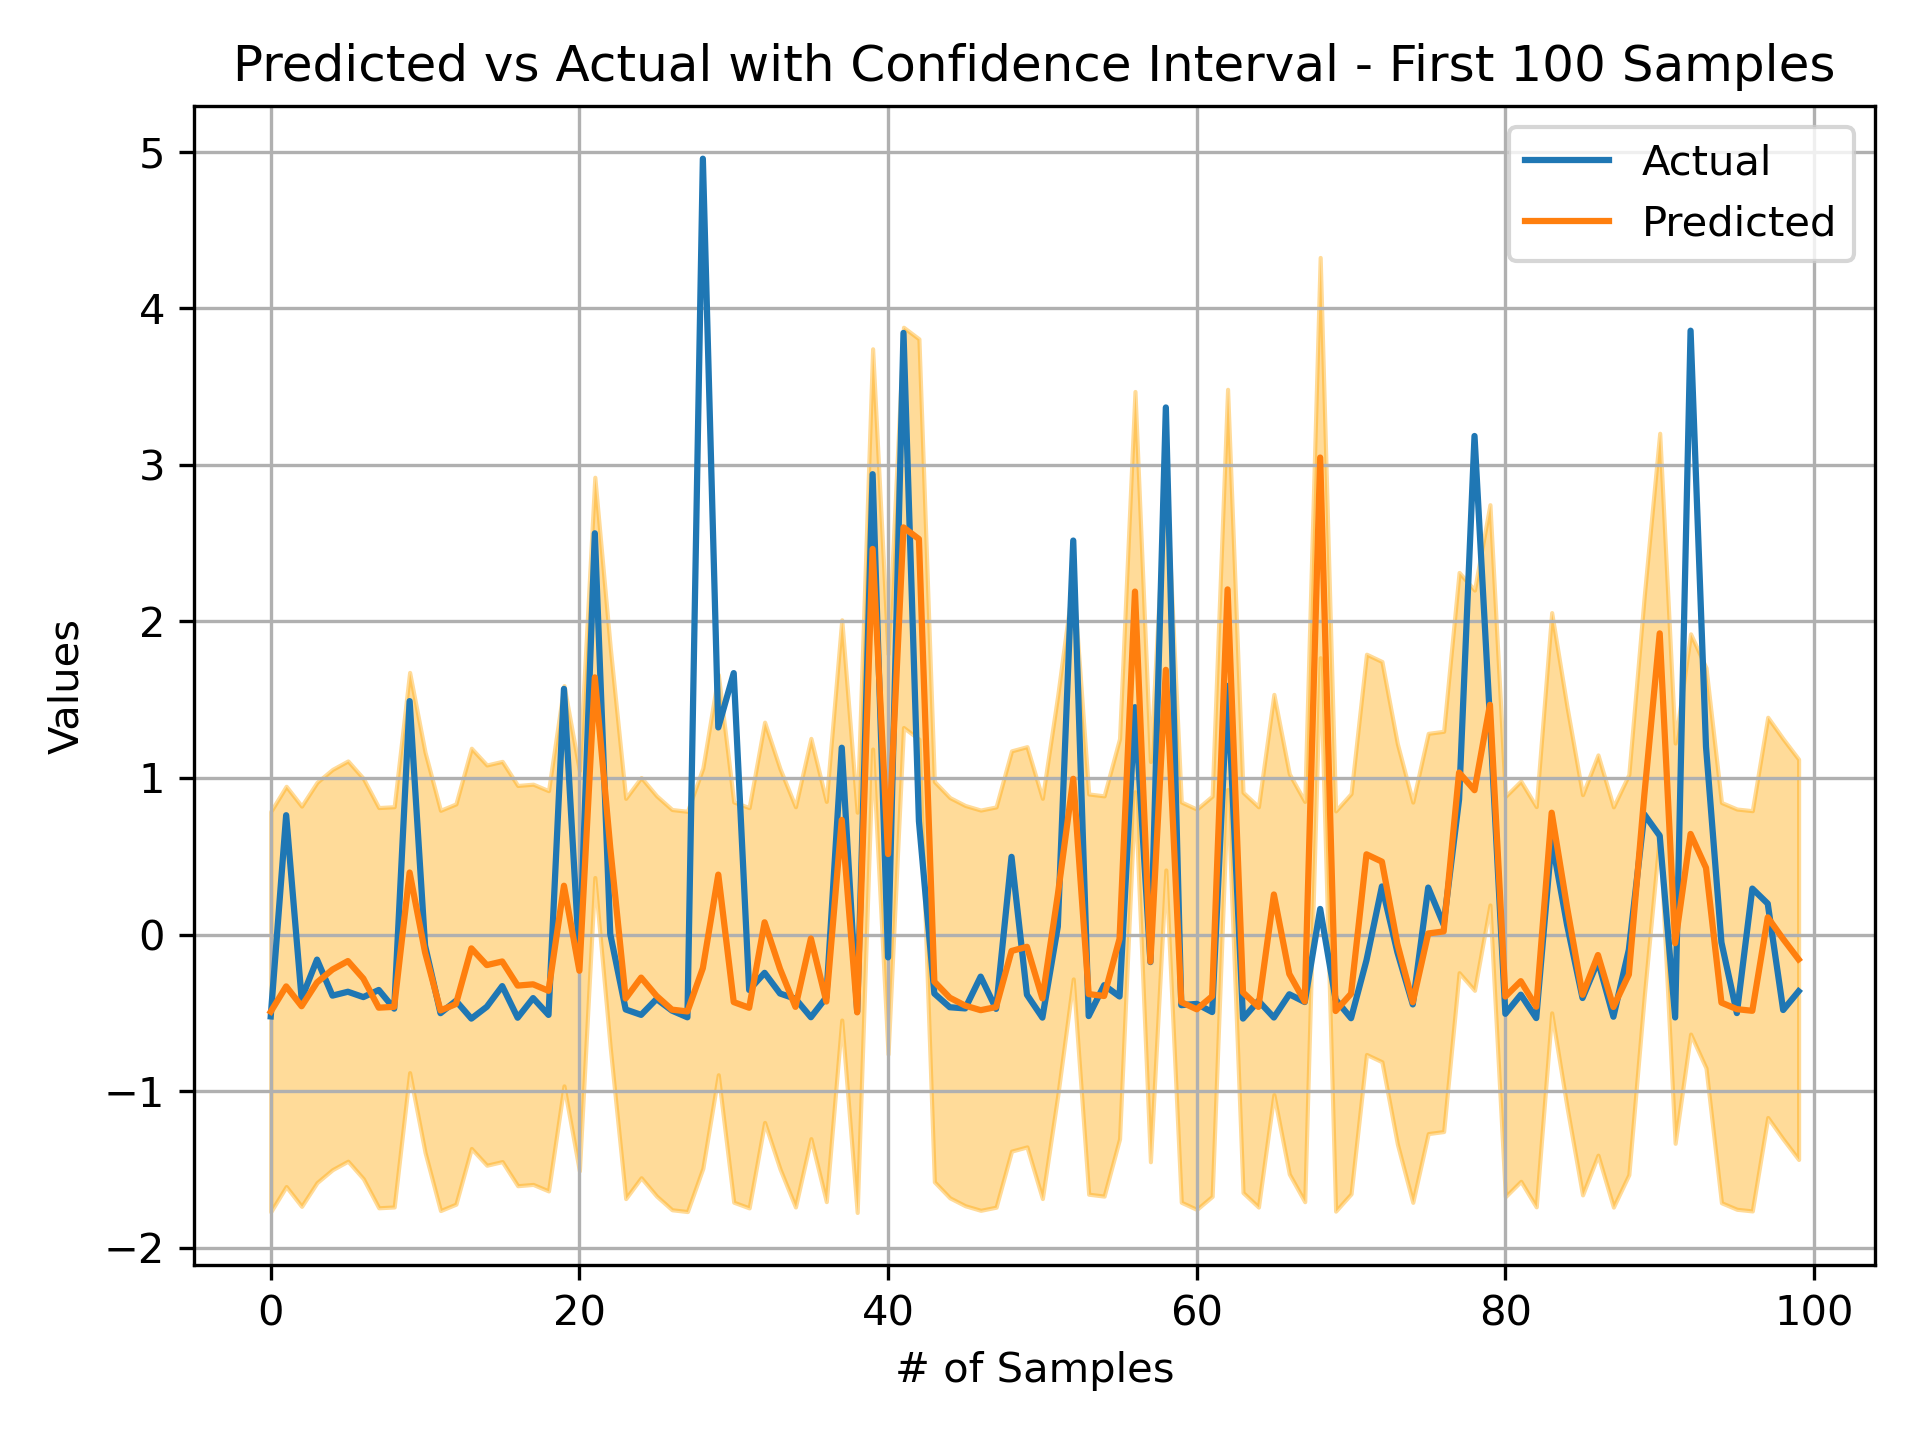
\includegraphics[width=1\linewidth]{docs//assets/regressor_predicted_vs_actual.png}
    \caption{Predicted vs Actual with Confidence Interval}
    \label{fig:rfg-ci}
\end{figure}

\subsection{Conclusion}

In conclusion, the regression analysis conducted in Phase 2 of this project reveals significant insights into the prediction of \texttt{installCount}. Initially, a multiple linear regression model using the \texttt{statsmodel.OLS} was employed. Despite the high F-statistics, the model exhibited a low $R^2$ value and an increasing MSE, indicating a poor fit. The backward step-wise analysis, intended to improve the model by removing features with high p-values, did not yield a significant increase in the $R^2$ value or a decrease in MSE.

In response to these limitations, the project pivoted to a Random Forest Regressor, which demonstrated a marked improvement over the linear model. The tree-based approach resulted in a higher $R^2$ value, indicating a better fit for the dataset. The implementation of K-Fold cross-validation addressed potential overfitting issues, as evidenced by the low and consistent MSE scores across different folds.

The graphical analysis, including the plot of actual versus predicted values and the comparison within confidence intervals, further substantiates the Random Forest Regressor's effectiveness. These visuals show a more accurate and reliable prediction of installCount compared to the linear regression model.

Overall, the transition from a linear to a tree-based model in this analysis underscores the importance of model selection in data analysis. The Random Forest Regressor, with its ability to handle a large number of features and its resistance to overfitting, proved to be a more suitable choice for predicting installCount, offering both higher accuracy and reliability.

\bibliographystyle{apacite}
\bibliography{docs/tex/ref}
% \renewcommand{\arraystretch}{1.5} % Adjust to your needs
% \begin{adjustbox}{width=\textwidth,center}
% \begin{tabular}{cccccc|c}
% Classifier & Precision & Recall & Specificity & F1 Score & AUC & Confusion Matrix \\
% Decision Tree Pre-pruning & 0.804 & 0.770 & 0.812 & 0.786 & 0.791 & $\begin{matrix} 13032 & 3020 \\ 3699 & 12352 \end{matrix}$ \\
% Decision Tree Post-pruning & 0.812 & 0.727 & 0.831 & 0.767 & 0.779 & $\begin{matrix} 13345 & 2707 \\ 4381 & 11670 \end{matrix}$ \\
% Logistic Regression & 0.864 & 0.641 & 0.899 & 0.736 & 0.770 & $\begin{matrix} 14437 & 1615 \\ 5756 & 10295 \end{matrix}$ \\
% K-Nearest Neighbors & 0.835 & 0.620 & 0.878 & 0.711 & 0.749 & $\begin{matrix} 14089 & 1963 \\ 6104 & 9947 \end{matrix}$ \\
% Support Vector Machine & 0.875 & 0.672 & 0.904 & 0.760 & 0.788 & $\begin{matrix} 14515 & 1537 \\ 5263 & 10788 \end{matrix}$ \\
% Naive Bayes & 0.918 & 0.442 & 0.960 & 0.597 & 0.701 & $\begin{matrix} 15415 & 637 \\ 8954 & 7097 \end{matrix}$ \\
% Random Forest Bagging & 0.793 & 0.793 & 0.792 & 0.793 & 0.793 & $\begin{matrix} 12719 & 3333 \\ 3320 & 12731 \end{matrix}$ \\
% Stacking & 0.846 & 0.729 & 0.867 & 0.783 & 0.798 & $\begin{matrix} 13921 & 2131 \\ 4346 & 11705 \end{matrix}$ \\
% Boosting & 0.817 & 0.764 & 0.829 & 0.790 & 0.797 & $\begin{matrix} 13313 & 2739 \\ 3782 & 12269 \end{matrix}$ \\
% Neural Network & 0.824 & 0.767 & 0.836 & 0.794 & 0.802 & $\begin{matrix} 13422 & 2630 \\ 3740 & 12311 \end{matrix}$ \\
% \end{tabular}
% \end{adjustbox}

% \begin{center}
% \begin{tabular}{lclc}
% \toprule
% \textbf{Dep. Variable:}       &   installCount   & \textbf{  R-squared:         } &      0.368   \\
% \textbf{Model:}               &       OLS        & \textbf{  Adj. R-squared:    } &      0.368   \\
% \textbf{Method:}              &  Least Squares   & \textbf{  F-statistic:       } &  1.068e+04   \\
% \textbf{Date:}                & Thu, 30 Nov 2023 & \textbf{  Prob (F-statistic):} &      0.00    \\
% \textbf{Time:}                &     21:26:44     & \textbf{  Log-Likelihood:    } & -1.5240e+05  \\
% \textbf{No. Observations:}    &      128408      & \textbf{  AIC:               } &  3.048e+05   \\
% \textbf{Df Residuals:}        &      128400      & \textbf{  BIC:               } &  3.049e+05   \\
% \textbf{Df Model:}            &           7      & \textbf{                     } &              \\
% \textbf{Covariance Type:}     &    nonrobust     & \textbf{                     } &              \\
% \bottomrule
% \end{tabular}

% \begin{tabular}{lcccccc}
%                               & \textbf{coef} & \textbf{std err} & \textbf{t} & \textbf{P$> |$t$|$} & \textbf{[0.025} & \textbf{0.975]}  \\
% \midrule
% \textbf{const}                &      -0.0412  &        0.003     &   -15.422  &         0.000        &       -0.046    &       -0.036     \\
% \textbf{ratingCount}          &       0.5932  &        0.002     &   247.041  &         0.000        &        0.588    &        0.598     \\
% \textbf{sizeInMB}             &       0.0299  &        0.002     &    12.429  &         0.000        &        0.025    &        0.035     \\
% \textbf{lastUpdateAgeInDays}  &      -0.0734  &        0.002     &   -30.001  &         0.000        &       -0.078    &       -0.069     \\
% \textbf{appAgeInDays}         &       0.0702  &        0.002     &    28.752  &         0.000        &        0.065    &        0.075     \\
% \textbf{rating}               &      -0.0118  &        0.002     &    -5.237  &         0.000        &       -0.016    &       -0.007     \\
% \textbf{isInAppPurchases}     &       0.1568  &        0.005     &    30.019  &         0.000        &        0.147    &        0.167     \\
% \textbf{minAndroidVersion\_7} &      -0.1097  &        0.020     &    -5.503  &         0.000        &       -0.149    &       -0.071     \\
% \bottomrule
% \end{tabular}
% \begin{tabular}{lclc}
% \textbf{Omnibus:}       & 73565.243 & \textbf{  Durbin-Watson:     } &      1.995   \\
% \textbf{Prob(Omnibus):} &    0.000  & \textbf{  Jarque-Bera (JB):  } & 2705960.736  \\
% \textbf{Skew:}          &    2.156  & \textbf{  Prob(JB):          } &       0.00   \\
% \textbf{Kurtosis:}      &   25.072  & \textbf{  Cond. No.          } &       11.3   \\
% \bottomrule
% \end{tabular}
% %\caption{OLS Regression Results}
% \end{center}
% Notes: \newline
%  [1] Standard Errors assume that the covariance matrix of the errors is correctly specified.


% \renewcommand{\arraystretch}{3} % Adjust 1.5 to your needs
% \begin{adjustbox}{width=\textwidth,center}
% \begin{tabular}{ccccccc}
% Classifier & Confusion Matrix & Precision & Recall & Specificity & F1 Score & AUC \\
% Decision Tree Pre-pruning & $\begin{bmatrix} 13032 & 3020 \\ 3699 & 12352 \end{bmatrix}$ & 0.804 & 0.770 & 0.812 & 0.786 & 0.791 \\
% Decision Tree Post-pruning & $\begin{bmatrix} 13345 & 2707 \\ 4381 & 11670 \end{bmatrix}$ & 0.812 & 0.727 & 0.831 & 0.767 & 0.779 \\
% Logistic Regression & $\begin{bmatrix} 14437 & 1615 \\ 5756 & 10295 \end{bmatrix}$ & 0.864 & 0.641 & 0.899 & 0.736 & 0.770 \\
% K-Nearest Neighbors & $\begin{bmatrix} 14089 & 1963 \\ 6104 & 9947 \end{bmatrix}$ & 0.835 & 0.620 & 0.878 & 0.711 & 0.749 \\
% Support Vector Machine & $\begin{bmatrix} 14515 & 1537 \\ 5263 & 10788 \end{bmatrix}$ & 0.875 & 0.672 & 0.904 & 0.760 & 0.788 \\
% Naive Bayes & $\begin{bmatrix} 15415 & 637 \\ 8954 & 7097 \end{bmatrix}$ & 0.918 & 0.442 & 0.960 & 0.597 & 0.701 \\
% Random Forest Bagging & $\begin{bmatrix} 12719 & 3333 \\ 3320 & 12731 \end{bmatrix}$ & 0.793 & 0.793 & 0.792 & 0.793 & 0.793 \\
% Stacking & $\begin{bmatrix} 13921 & 2131 \\ 4346 & 11705 \end{bmatrix}$ & 0.846 & 0.729 & 0.867 & 0.783 & 0.798 \\
% Boosting & $\begin{bmatrix} 13313 & 2739 \\ 3782 & 12269 \end{bmatrix}$ & 0.817 & 0.764 & 0.829 & 0.790 & 0.797 \\
% Neural Network & $\begin{bmatrix} 13422 & 2630 \\ 3740 & 12311 \end{bmatrix}$ & 0.824 & 0.767 & 0.836 & 0.794 & 0.802 \\
% \end{tabular}
% \end{adjustbox}


\newpage
% \bibliographystyle{apacite}
% \bibliography{references} % Your references.bib file

\end{document}
